% Copyright (c) 2015 Daniele Masini - d.masini.it@gmail.com

\section{Esercizi}
\subsection{Esercizi dei singoli paragrafi}

\begingroup
\hypersetup{linkcolor=black}
\subsubsection*{\ref{sect:metodo_assiomatico_concetti_primitivi} - 
\nameref{sect:metodo_assiomatico_concetti_primitivi}}
\endgroup

\begin{esercizio}
\label{ese:1.1}
Quali delle seguenti frasi sono proposizioni logiche?
\begin{enumeratea}
\item <<I matematici sono intelligenti>>\tab\tab\qquad\boxV\quad\boxF
\item <<12 è un numero dispari>>\tab\tab\tab\qquad\boxV\quad\boxF
\item <<Pascoli è stato un grande poeta>>\tab\tab\qquad\boxV\quad\boxF
\item <<Pascoli ha scritto La Divina 
Commedia>>\tab\qquad\boxV\quad\boxF
\item <<Pascoli ha scritto poesie>>\tab\tab\tab\qquad\boxV\quad\boxF
\item <<Lucia è una bella ragazza>>\tab\tab\tab\qquad\boxV\quad\boxF
\item <<Lucia ha preso 8 al compito di 
matematica>>\tab\qquad\boxV\quad\boxF
\item <<Che bella serata!>>\tab\tab\tab\tab\qquad\boxV\quad\boxF
\item <<Il rombo è una figura 
storta>>\tab\tab\tab\qquad\boxV\quad\boxF
\item <<Per favore fate silenzio!>>\tab\tab\tab\qquad\boxV\quad\boxF
\item <<$2+2=5$>>\tab\tab\tab\tab\tab\qquad\boxV\quad\boxF
\item <<I miei insegnanti sono tutti 
laureati>>\tab\tab\qquad\boxV\quad\boxF
\end{enumeratea}
\end{esercizio}

\begin{esercizio}
\label{ese:1.2}
A partire dalle due proposizioni $p =\;$<<16 è divisibile per 2>> e 
$q =\;$<<16 è divisibile per 4>>, costruisci le proposizioni $p\vee q$ 
e $p\wedge q$.
\end{esercizio}

\begin{esercizio}
\label{ese:1.3}
A partire dalle proposizioni $p=\;$<<18 è divisibile per 3>> e 
$q=\;$<<18 è numero dispari>> costruisci le proposizioni di seguito 
indicate e stabilisci il loro valore di verità
\begin{multicols}{2}
\begin{enumeratea}
\item $p\vee q$			\tab\tab\qquad\boxV\quad\boxF
\item $p\wedge q$		\tab\tab\qquad\boxV\quad\boxF
\item $\neg p$			\tab\tab\qquad\boxV\quad\boxF
\item $\neg q$			\tab\tab\qquad\boxV\quad\boxF
\item $p\vee \neg q$		\tab\tab\qquad\boxV\quad\boxF
\item $\neg p\wedge q$	\tab\tab\qquad\boxV\quad\boxF
\item $p\wedge \neg q$	\tab\tab\qquad\boxV\quad\boxF
\item $\neg p\vee\neg q$		\tab\qquad\boxV\quad\boxF
\item $\neg p\wedge\neg q$	\tab\qquad\boxV\quad\boxF
\item $\neg (p\wedge q)$		\tab\qquad\boxV\quad\boxF
\end{enumeratea}
\end{multicols}
\end{esercizio}

\begin{esercizio}
\label{ese:1.4}
A partire dalle proposizioni $a=\;$<<20 è minore di 10>>, $b=\;$<<20 
è maggiore di 1>>, $c=\;$<<20 è multiplo di 5>>, $d=\;$<<20 è 
dispari>>, stabilisci il valore di verità delle seguenti proposizioni:
\begin{multicols}{2}
\begin{enumeratea}
\item $a\vee b$						
\tab\tab\tab\boxV\quad\boxF
\item $a\wedge c$					
\tab\tab\tab\boxV\quad\boxF
\item $d\wedge a$					
\tab\tab\tab\boxV\quad\boxF
\item $\neg a \wedge b$				
\tab\tab\tab\boxV\quad\boxF
\item $a\vee \neg b$					
\tab\tab\tab\boxV\quad\boxF
\item $\neg b\wedge \neg a$				
\tab\tab\boxV\quad\boxF
\item $(\neg a\wedge \neg b)\vee(c\wedge d)$	\tab\boxV\quad\boxF
\item $(a\vee \neg b)\wedge(c \vee \neg d)$	\tab\boxV\quad\boxF
\end{enumeratea}
\end{multicols}
\end{esercizio}

\begin{esercizio}
\label{ese:1.5}
Date le proposizioni $p=\;$<<Oggi è lunedì>> e $q=\;$<<Oggi studio 
matematica>>, scrivi in simboli le seguenti proposizioni:
\begin{enumeratea}
\item <<Oggi è lunedì e studio matematica>>
\item <<Oggi non è lunedì e studio matematica>>
\item <<Oggi è lunedì e non studio matematica>>
\item <<Oggi non è lunedì e non studio matematica>>
\end{enumeratea}
\end{esercizio}

\pagebreak

\begin{esercizio}
\label{ese:1.6}
In quale delle seguenti proposizioni è utilizzata la ``o'' inclusiva 
e in quali la ``o'' esclusiva?
\begin{enumeratea}
\item <<Nelle fermate a richiesta l'autobus si ferma se qualche 
persona deve scendere o salire>>
\item <<Luca sposerà Maria o Claudia>>
\item <<Fammi chiamare da Laura o da Elisa>>
\item <<Si raggiunge l'unanimità quando sono tutti favorevoli o tutti 
contrari>>
\item <<Vado al cinema con Carla o con Luisa>>
\item <<Per le vacanze andrò al mare o a Firenze>>
\end{enumeratea}
\end{esercizio}

\begin{esercizio}
\label{ese:1.7}
A partire dalle proposizioni $p=\;$<<Oggi pioverà>> e $\neg 
p=\;$<<Oggi non pioverà>>, scrivere le proposizioni $p\veebar \neg 
p$, $p\vee \neg p$, $p\wedge \neg p$. Scrivere quindi la loro tabella 
della verità.
\end{esercizio}

\begin{esercizio}
\label{ese:1.8}
Scrivere le tabelle di verità delle seguenti formule
\begin{multicols}{3}
\begin{enumeratea}
\item $p\wedge(p\vee q)$
\item $p\vee(p\wedge q)$
\item $p\veebar(p\wedge q)$
\item $p\wedge(p\veebar q)$
\item $(p\vee \neg q)\wedge (\neg p\vee q)$
\item $(p\vee q)\wedge q$
\item $(\neg p\vee q)\wedge (p\wedge q)$
\item $\neg(p\vee q)\wedge (p\vee \neg q)$
\item $(p\vee \neg q)\wedge \neg p$
\item $(\neg p\vee q)\wedge \neg q$
\item $(p\wedge q)\wedge \neg p$
\item $(p\vee r)\vee \neg q$
\end{enumeratea}
\end{multicols}
\end{esercizio}

\begin{esercizio}
\label{ese:1.9}
Costruisci la tavola di verità delle seguenti proposizioni
\begin{multicols}{3}
\begin{enumeratea}
\item $(\neg p\vee q)\wedge(p\wedge r)$
\item $\neg(p\vee q)\wedge(r\vee \neg q)$
\item $(p\vee\neg q)\wedge \neg r$
\item $p\vee\neg(r\veebar q)$
\item $(\neg p\veebar q)\wedge(r\vee q)$
\item $\neg(p\vee r)\wedge(r\veebar q)$
\item $(p\vee\neg q)\wedge\neg r$
\item $(\neg p\vee\neg q)\wedge(r\vee\neg q)$
\item $\neg((p\veebar q)\wedge \neg r)$
\end{enumeratea}
\end{multicols}
\end{esercizio}

\begin{esercizio}
\label{ese:1.10}
Verificare che, date due proposizioni $p$ e $q$, la proposizione 
composta $(\neg p\wedge q)\vee(p\wedge \neg q)$ è equivalente alla 
proposizione $p\veebar q$. Dimostrare l'equivalenza verificando che 
le tavole della verità sono uguali.
\end{esercizio}

\begin{esercizio}
\label{ese:1.11}
Se $p\wedge q$ è falso, quale dei seguenti enunciati è vero?
\begin{multicols}{4}
\begin{enumeratea}
\item $p\wedge \neg q$
\item $\neg p\wedge q$
\item $\neg p\wedge\neg q$
\item $\neg p\vee\neg q$
\end{enumeratea}
\end{multicols}
%Risposta [D]
\end{esercizio}

\begin{esercizio}
\label{ese:1.12}
Qual è la negazione della frase <<Ogni volta che ho preso l'ombrello 
non è piovuto>>?
\begin{enumeratea}
\item <<Almeno una volta sono uscito con l'ombrello ed è piovuto>>
\item <<Quando esco senza ombrello piove sempre>>
\item <<Tutti i giorni in cui non piove esco con l'ombrello>>
\item <<Tutti i giorni che è piovuto ho preso l'ombrello>>
\end{enumeratea}
\end{esercizio}

\begin{esercizio}
\label{ese:1.13}
Scrivi le negazioni delle seguenti frasi che contengono dei 
quantificatori:
\begin{enumeratea}
\item <<Al compito di matematica eravamo tutti presenti>>
\item <<Ogni giorno il professore ci dà compiti per casa>>
\item <<Ogni giorno Luca vede il telegiornale>>
\item <<Tutti i miei familiari portano gli occhiali>>
\item <<Tutti hanno portato i soldi per la gita>>
\end{enumeratea}
\end{esercizio}

\pagebreak

\begin{esercizio}
\label{ese:1.14}
Sono date le frasi $p=\;$<<Mario è cittadino romano>> e $q=\;$<<Mario 
è cittadino italiano>>, scrivi per esteso le seguenti implicazioni e 
indica quale di esse è vera.
\begin{multicols}{3}
\begin{enumeratea}
\item $p\Rightarrow q$		\tab\quad\boxV\quad\boxF
\item $q\Rightarrow p$		\tab\quad\boxV\quad\boxF
\item $q\Leftrightarrow p$	\tab\quad\boxV\quad\boxF
\end{enumeratea}
\end{multicols}
\end{esercizio}

\begin{esercizio}
\label{ese:1.15}
Trasforma nella forma <<Se \ldots{} allora \ldots{}>> le seguenti 
frasi:
\begin{enumeratea}
\item <<Un oggetto lanciato verso l'alto ricade a terra>>
\item <<Quando piove prendo l'ombrello>>
\item <<I numeri la cui ultima cifra è 0 sono divisibili per 5>>
\item <<Per essere promosso occorre aver raggiunto la sufficienza>>
\end{enumeratea}
\end{esercizio}

\begin{esercizio}
\label{ese:1.16}
Date le proposizioni $p$, $q$, e $r$ costruire la tavola di verità 
delle seguenti proposizioni
\begin{multicols}{3}
\begin{enumeratea}
\item $p\Rightarrow\neg q$
\item $\neg p\Rightarrow q$
\item $(p\vee q)\Rightarrow \neg q$
\item $p\Rightarrow (q\vee \neg q)$
\item $(p\wedge q)\Rightarrow(p\vee q)$
\item $p\vee(p\Rightarrow q)$
\item $(p\wedge q)\Rightarrow(\neg q\vee r)$
\item $(p\wedge q)\Leftrightarrow(\neg p\vee \neg q)$
\item $(p\Rightarrow q)\wedge \neg q$
\item $(p\Rightarrow q)\vee(q\Rightarrow p)$
\item $(\neg p\vee\neg q)\Leftrightarrow(p\wedge q)$
\item $\neg(\neg p\wedge r)\Leftrightarrow(q\vee\neg r)$
\end{enumeratea}
\end{multicols}
\end{esercizio}

\begin{esercizio}
\label{ese:1.17}
Completa i seguenti ragionamenti:
\begin{enumeratea}
\item <<Se un numero è multiplo di 10 allora è pari>>; <<il numero 
$n$ non è pari quindi \ldots\ldots\ldots\ldots>>
\item <<Se il sole tramonta fa buio>>; <<il sole è tramontato quindi 
\ldots\ldots\ldots\ldots>>
\end{enumeratea}
\end{esercizio}

\begin{esercizio}
\label{ese:1.18}
Distingui nelle seguenti frasi le definizioni dalle proposizioni o 
proprietà
\begin{enumeratea}
\item <<La Terra ruota su se stessa in un giorno>>		
			\hfill\boxD\quad\boxP
\item <<Il solstizio è il momento in cui il Sole raggiunge, nel suo 
moto apparente lungo l'eclittica, il punto di declinazione massima o 
minima>>			\hfill\boxD\quad\boxP
\item <<La cellula è l'unità fondamentale di tutti gli organismi 
viventi>>\hfill\boxD\quad\boxP
\item <<I virus sono responsabili di alcune 
malattie>>\hfill\boxD\quad\boxP
\item <<I numeri che hanno per ultima cifra 0 sono numeri 
pari>>\hfill\boxD\quad\boxP
\item <<Un numero si dice pari se è divisibile per 
2>>\hfill\boxD\quad\boxP
\end{enumeratea}
\end{esercizio}

\begin{esercizio}
\label{ese:1.19}
Dimostra con un controesempio che l'affermazione <<Tutti i multipli 
di 3 sono dispari>> non è vera.
\end{esercizio}

\begin{esercizio}[I Giochi di Archimede, 2011]
\label{ese:1.20}
Dopo una rissa in campo l'arbitro vuole espellere il capitano di una 
squadra di calcio. \`E uno tra Paolo, Andrea e Gabriele ma, siccome 
nessuno ha la fascia al braccio, non sa qual è dei tre. Paolo dice di 
non essere il capitano; Andrea dice che il capitano è Gabriele; 
Gabriele dice che il capitano è uno degli altri due. Sapendo che uno 
solo dei tre dice la verità, quale delle affermazioni seguenti è 
sicuramente vera?
\begin{enumeratea}
\item Gabriele non è il capitano;
\item Andrea dice la verità;
\item Paolo dice la verità;
\item Andrea è il capitano;
\item Gabriele mente.
\end{enumeratea}
\end{esercizio}

\begin{esercizio}[Giochi d'autunno, 2010]
\label{ese:1.21}
Ecco le dichiarazioni rilasciate da quattro amiche:\\
Anna: <<Io sono la più anziana>>;\\
Carla: <<Io non sono né la più giovane né la più anziana>>;\\
Liliana: <<Io non sono la più giovane>>;\\
Milena: <<Io sono la più giovane>>.\\
Il fatto è che una di loro (e solo una) ha mentito. Chi è, delle 
quattro amiche, effettivamente la più giovane?
\end{esercizio}

\begin{esercizio}[I Giochi di Archimede, 2010]
\label{ese:1.22}
Un celebre investigatore sta cercando il colpevole di un omicidio tra 
cinque sospettati: Anna, Bruno, Cecilia, Dario ed Enrico. Egli sa che 
il colpevole mente sempre e gli altri dicono sempre la verità. Anna 
afferma: <<Il colpevole è un maschio>>, Cecilia dice: <<\`E stata 
Anna oppure è stato Enrico>>. Infine Enrico dice: <<Se Bruno è 
colpevole allora Anna è innocente>>. Chi ha commesso l'omicidio?
\end{esercizio}

\begin{esercizio}[I Giochi di Archimede, 2009]
\label{ese:1.23}
Quattro amici, Anna, Bea, Caio e Dino, giocano a poker con 20 carte 
di uno stesso mazzo: i quattro re, le quattro regine, i quattro fanti, 
i quattro assi e i quattro dieci. Vengono distribuite cinque carte a 
testa. Anna dice: <<Io ho un poker!>> (quattro carte dello stesso 
valore). Bea dice: <<Io ho tutte e cinque le carte di cuori>>. Caio 
dice: <<Io ho cinque carte rosse>>. Infine Dino dice: <<Io ho tre 
carte di uno stesso valore e anche le altre due hanno lo stesso 
valore>>. Sappiamo che una e una sola delle affermazioni è falsa; chi 
sta mentendo?
\end{esercizio}

\begin{esercizio}[I Giochi di Archimede, 2008]
\label{ese:1.24}
Un satellite munito di telecamera inviato sul pianeta Papilla ha 
permesso di stabilire che è falsa la convinzione di qualcuno che: 
<<su Papilla sono tutti grassi e sporchi>>. Quindi adesso sappiamo 
che:
\begin{enumeratea}
\item <<su Papilla almeno un abitante è magro e pulito>>;
\item <<su Papilla tutti gli abitanti sono magri e puliti>>;
\item <<almeno un abitante di Papilla è magro>>;
\item <<almeno un abitante di Papilla è pulito>>;
\item <<se su Papilla tutti gli abitanti sono sporchi, almeno uno di 
loro è magro>>.
\end{enumeratea}
\end{esercizio}

\begin{esercizio}[I Giochi di Archimede, 2000]
\label{ese:1.25}
Anna, Barbara, Chiara e Donatella si sono sfidate in una gara di 
nuoto fino alla boa. All'arrivo non ci sono stati ex-equo. Al ritorno, 
Anna dice: <<Chiara è arrivata prima di Barbara>>; Barbara dice: 
<<Chiara è arrivata prima di Anna>>; Chiara dice: <<Io sono arrivata 
seconda>>. Sapendo che una sola di esse ha detto la verità
\begin{enumeratea}
\item si può dire solo chi ha vinto, 
\item si può dire solo chi è arrivata seconda, 
\item si può dire solo chi è arrivata terza, 
\item si può dire solo chi è arrivata ultima, 
\item non si può stabile la posizione in classifica di nessuna. 
\end{enumeratea}
\end{esercizio}

\begin{esercizio}[I Giochi di Archimede, 1999]
\label{ese:1.26}
<<In ogni scuola c'è almeno una classe in cui sono tutti promossi>>. 
Volendo negare questa affermazione, quale dei seguenti enunciati 
sceglieresti?
\begin{enumeratea}
\item <<In ogni scuola c'è almeno una classe in cui sono tutti 
bocciati>>;
\item <<In ogni scuola c'è almeno un bocciato in tutte le classi;
\item <<C'è almeno una scuola che ha almeno un bocciato in ogni 
classe>>;
\item <<C'è almeno una scuola in cui c'è una classe che ha almeno un 
bocciato>>.
\end{enumeratea}
\end{esercizio}

\begin{esercizio}[I Giochi di Archimede, 1998]
\label{ese:1.27}
Su un isola vivono tre categorie di persone: i cavalieri, che dicono 
sempre la verità, i furfanti, che mentono sempre, ed i paggi che dopo 
una verità dicono sempre una menzogna e viceversa. Sull'isola 
incontro un vecchio, un ragazzo e una ragazza. Il vecchio afferma: 
<<Io sono paggio>> e <<Il ragazzo è cavaliere>>. Il ragazzo dice: <<Io 
sono cavaliere>> e <<La ragazza è paggio>>. La ragazza afferma infine: 
<<Io sono furfante>> e <<Il vecchio è paggio>>. Si può allora 
affermare che:
\begin{enumeratea}
\item c'è esattamente un paggio;
\item ci sono esattamente due paggi;
\item ci sono esattamente tre paggi;
\item non c'è alcun paggio;
\item il numero dei paggi non è sicuro.
\end{enumeratea}
\end{esercizio}

\begin{esercizio}[I Giochi di Archimede, 1997]
\label{ese:1.28}
<<Se il pomeriggio ho giocato a tennis, la sera ho fame e se la sera 
ho fame, allora mangio troppo>>. Quale delle seguenti conclusioni non 
posso trarre da queste premesse?
\begin{enumeratea}
\item <<Se gioco a tennis il pomeriggio, allora la sera ho fame e 
mangio troppo>>;
\item <<Se la sera ho fame, allora mangio troppo, oppure ho giocato a 
tennis il pomeriggio>>;
\item <<Se la sera non ho fame, allora non ho giocato a tennis il 
pomeriggio>>;
\item <<Se la sera non ho fame, allora non mangio troppo>>;
\item <<Se la sera non mangio troppo, allora non ho giocato a tennis 
il pomeriggio>>.
\end{enumeratea}
\end{esercizio}

\begin{esercizio}
\label{ese:1.29}
Dimostra che in ogni festa c'è sempre una coppia di persone che balla 
con lo stesso numero di invitati.
\end{esercizio}

\begin{esercizio}
\label{ese:1.30}
Mr.~Smith, Mr.~Taylor e Mr.~Elder insegnano 6 diverse materie 
(Biologia, Geografia, Matematica, Storia, Inglese e Fisica), ciascuno 
di essi due materie. Abbiamo le seguenti informazioni: Gli insegnanti 
di Fisica ed Inglese sono vicini di casa; Mr.~Smith è il più giovane 
dei tre. Mr.~Elder gioca a poker con l'insegnante d'Inglese e con 
quello di Biologia ogni domenica. L'insegnante di Biologia è più 
vecchio di quello di Matematica. L'insegnante di Geografia, quello di 
Matematica e Mr.~Smith andranno a fare un giro in bici il prossimo 
weekend. Associare ogni insegnante alle materie che insegna.
% [Sm: S e F; T: B e I; E: G e M].
\end{esercizio}

\begin{esercizio}[Test di ammissione a Ingegneria 1999]
\label{ese:1.31}
In una squadra di calcio giocano Amilcare, Bertoldo e Carletto nei 
ruoli di portiere, centravanti, libero (non necessariamente in 
quest'ordine). Si sa che:
\begin{enumerate}
\item Il centravanti è il più basso di statura ed è scapolo;
\item Amilcare è il suocero di Carletto ed è più alto del portiere.
\end{enumerate}
Quale delle seguenti affermazioni è necessariamente vera?
\begin{multicols}{2}
\begin{enumeratea}
\item Bertoldo è il genero di Carletto;
\item Bertoldo ha sposato la sorella di Carletto;
\item Carletto è il portiere;
\item Carletto è scapolo;
\item Amilcare è il centravanti.
\end{enumeratea}
\end{multicols}
\end{esercizio}

\begin{esercizio}[Test di ammissione a Medicina 1997]
\label{ese:1.32}
Un alano, un boxer, un collie e un dobermann vincono i primi 4 premi 
ad una mostra canina. I loro padroni sono il Sig.~Estro, il 
Sig.~Forti, il Sig.~Grassi ed il Sig.~Rossi, non necessariamente in 
quest'ordine. I nomi dei cani sono Jack, Kelly, Lad, Max, non 
necessariamente in quest'ordine. Disponiamo inoltre delle seguenti 
informazioni:
\begin{enumerate*}
\item cane del Sig.~Grassi non ha vinto né il primo, né il secondo 
premio;
\item il collie ha vinto il primo premio;
\item Max ha vinto il secondo premio;
\item l'alano si chiama Jack;
\item il cane del Sig.~Forti, il dobermann, ha vinto il quarto premio;
\item il cane del Sig.~Rossi si chiama Kelly.
\end{enumerate*}
Da quale cane è stato vinto il primo premio?
\begin{multicols}{2}
\begin{enumeratea}
\item Il cane del Sig.~Estro
\item Il cane del Sig.~Rossi
\item Max
\item Jack
\item Lad
\end{enumeratea}
\end{multicols}
\end{esercizio}

\begingroup
\hypersetup{linkcolor=black}
\subsubsection*{\ref{sect:enti_fondamentali} - 
\nameref{sect:enti_fondamentali}}
\endgroup

\begin{esercizio}
\label{ese:1.33}
Gli enti primitivi della geometria sono quelli...
\begin{enumeratea}
\item che occorre definire;
\item che occorre dimostrare;
\item che non si definiscono;
\item che si conoscono già per averli studiati prima.
\end{enumeratea}
\end{esercizio}

\begin{esercizio}
\label{ese:1.34}
Gli assiomi sono:
\begin{enumeratea}
\item proposizioni note che si preferisce non dimostrare per non 
appesantire lo studio;
\item proposizioni che è necessario dimostrare;
\item proposizioni che si assumono vere senza dimostrazione;
\item proposizioni che non si definiscono;
\item proposizioni che non si dimostrano perché la loro dimostrazione 
è molto semplice.
\end{enumeratea}
\end{esercizio}
	
\begin{esercizio}
\label{ese:1.35}
Quali delle seguenti affermazioni sono vere?
\begin{enumeratea}
\item Due punti sono sempre allineati		
\tab\tab\tab\tab\boxV\quad\boxF
\item Tre punti sono sempre allineati		
\tab\tab\tab\tab\boxV\quad\boxF
\item Tre punti sono sempre complanari		
\tab\tab\tab\tab\boxV\quad\boxF
\item Tre punti allineati individuano un unico piano	
\tab\tab\boxV\quad\boxF
\item Una retta e un punto esterno ad essa individuano un piano 
\tab\boxV\quad\boxF
\end{enumeratea}
\end{esercizio}

\begin{esercizio}
\label{ese:1.36}
Su una retta si segnano quattro punti $A$, $B$, $C$ e $D$. Quanti 
segmenti restano individuati?
\end{esercizio}

\begin{esercizio}
\label{ese:1.37}
Date tre semirette $a$, $b$ e $c$ aventi la stessa origine $O$, 
quanti angoli restano individuati?
\end{esercizio}

\begin{esercizio}
\label{ese:1.38}
Unisci in tutti i modi possibili, mediante delle rette, tre punti non 
allineati e posti sullo stesso piano.
\end{esercizio}

\begin{esercizio}
\label{ese:1.39}
Unisci in tutti i modi possibili, mediante delle rette, quattro 
punti, a tre a tre non allineati, di uno stesso piano.
\end{esercizio}

\begin{esercizio}
\label{ese:1.40}
Quattro rette a due a due incidenti quanti punti di intersezione 
individuano complessivamente?
\end{esercizio}

\begin{esercizio}
\label{ese:1.41}
Quale assioma è rappresentato nella figura~\ref{fig:ese1.41}?
\begin{enumeratea}
\item tre punti distinti non allineati determinano uno ed un solo 
piano che li contiene;
\item su un piano esistono infiniti punti ed infinite rette;
\item la retta passante per due punti distinti di un piano giace 
completamente nel piano;
\item su una retta esistono infiniti punti.
\end{enumeratea}
\end{esercizio}


\begin{inaccessibleblock}[Figura: TODO]
 \begin{figure}[htb]
 \centering% Copyright (c) 2015 Daniele Masini - d.masini.it@gmail.com

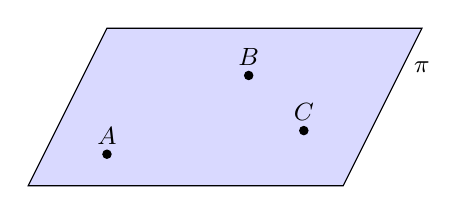
\begin{tikzpicture}[scale=1,font=\small]
\usetikzlibrary{calc}

\begin{scope}
\draw[fill, blue!15] (0,0) -- (1,2) -- (5,2) -- (4,0) -- cycle;
\draw (0,0) -- (1,2) -- (5,2) -- (4,0) -- cycle;
\coordinate (a) at (1,0.4);
\coordinate (b) at (2.8,1.4);
\coordinate (c) at (3.5,.7);
\draw[fill] (a) circle (1.5pt) node[above] {$A$};
\draw[fill] (b) circle (1.5pt) node[above] {$B$};
\draw[fill] (c) circle (1.5pt) node[above] {$C$};
\node at (5,1.5) {$\pi$};

\end{scope}

\end{tikzpicture}

 \caption{Esercizio \ref{ese:1.41}}\label{fig:ese1.41}
\end{figure}
\end{inaccessibleblock}

\begin{esercizio}
\label{ese:1.42}
Rispondi a voce alle seguenti domande
\begin{enumeratea}
\item Qual è l'origine della parola ``geometria''?
\item Qual è la differenza tra ``assioma'' e ``teorema''?
\item Qual è la differenza tra ``ente definito'' e ``ente primitivo''?
\end{enumeratea}
\end{esercizio}

\begingroup
\hypersetup{linkcolor=black}
\subsubsection*{\ref{sect:prime_definizioni} - 
\nameref{sect:prime_definizioni}}
\endgroup

\begin{esercizio}
\label{ese:1.43}
Disegna una retta $a$ e una retta $b$ che si incontrano in un punto 
$X$, disegna anche una retta $c$ che incontra la $a$ in $Y$ e la $b$ 
in $Z$. Elenca tutte le semirette e tutti i segmenti che si vengono a 
formare.
\end{esercizio}

\begin{esercizio}
\label{ese:1.44}
Disegna due rette $a$ e $b$ parallele tra di loro; disegna poi la 
retta $c$ che interseca la $a$ in $A$ e la $b$ in $B$; disegna poi la 
retta $d$ che interseca $a$ in $A$ e $b$ in $C$. Quali segmenti si 
vengono a formare?
\end{esercizio}

\begin{esercizio}
\label{ese:1.45}
Rappresenta graficamente ciascuna delle seguenti situazioni:
\begin{enumeratea}
\item $A\in r$~~e~~$B\in r$,~~$B\in s$~~e~~$C\in s$,~~$A\in 
t$~~e~~$C\in t$
\item $AB\subset r$,~~$CD\subset r$,~~$AB\cap CD=AD$.~~$AB\cup 
CD=\ldots{}$
\item $AB\subset r$,~~$CD\subset r$,~~$AB\cap CD=\emptyset$.~~$AB\cup 
CD=\ldots{}$
\item $AB\subset r$,~~$CD\subset s$,~~$r\parallel s$,~~$P\notin r\cup 
s$
\end{enumeratea}
\end{esercizio}

\begin{esercizio}
\label{ese:1.46}
Attribuisci il nome corretto a ciascuna coppia di segmenti 
rappresentati nella figura~\ref{fig:ese1.46} tra: adiacenti, 
incidenti, disgiunti, consecutivi.
\end{esercizio}


\begin{inaccessibleblock}[Figura: TODO]
 \begin{figure}[htb]
 \centering% Copyright (c) 2015 Daniele Masini - d.masini.it@gmail.com

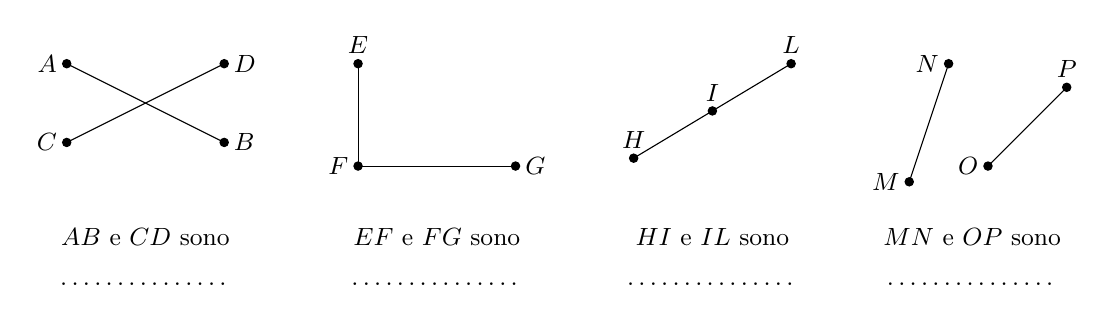
\begin{tikzpicture}[scale=1,font=\small]
\usetikzlibrary{calc}

\begin{scope}
\coordinate (a) at (0,0);
\coordinate (b) at (2,-1);
\coordinate (c) at (0,-1);
\coordinate (d) at (2,0);
\draw (a) node[left] {$A$} -- (b) node[right] {$B$};
\draw (c) node[left] {$C$} -- (d) node[right] {$D$};
\draw[fill] (a) circle (1.5pt) (b) circle (1.5pt) (c) circle (1.5pt) (d) circle (1.5pt);
\node at (1,-2.2) {$AB$ e $CD$ sono};
\node at (1,-2.8) {\ldots\ldots\ldots\ldots\ldots};
\end{scope}

\begin{scope}[xshift=3.7cm]
\coordinate (e) at (0,0);
\coordinate (f) at (0,-1.3);
\coordinate (g) at (2,-1.3);
\draw (e) node[above] {$E$} -- (f) node[left] {$F$} -- (g) node[right] {$G$};
\draw[fill] (e) circle (1.5pt) (f) circle (1.5pt) (g) circle (1.5pt);
\node at (1,-2.2) {$EF$ e $FG$ sono};
\node at (1,-2.8) {\ldots\ldots\ldots\ldots\ldots};
\end{scope}

\begin{scope}[xshift=7.2cm]
\coordinate (h) at (0,-1.2);
\coordinate (i) at (1,-0.6);
\coordinate (l) at (2,0);
\draw (h) node[above] {$H$} -- (i) node[above] {$I$} -- (l) node[above] {$L$};
\draw[fill] (h) circle (1.5pt) (i) circle (1.5pt) (l) circle (1.5pt);
\node at (1,-2.2) {$HI$ e $IL$ sono};
\node at (1,-2.8) {\ldots\ldots\ldots\ldots\ldots};
\end{scope}

\begin{scope}[xshift=10.7cm]
\coordinate (m) at (0,-1.5);
\coordinate (n) at (0.5,0);
\coordinate (o) at (1,-1.3);
\coordinate (p) at (2,-0.3);
\draw (m) node[left] {$M$} -- (n) node[left] {$N$};
\draw (o) node[left] {$O$} -- (p) node[above] {$P$};
\draw[fill] (m) circle (1.5pt) (n) circle (1.5pt) (o) circle (1.5pt) (p) circle (1.5pt);
\node at (0.8,-2.2) {$MN$ e $OP$ sono};
\node at (0.8,-2.8) {\ldots\ldots\ldots\ldots\ldots};
\end{scope}

\end{tikzpicture}

 \caption{Esercizio \ref{ese:1.46}}\label{fig:ese1.46}
\end{figure}
\end{inaccessibleblock}

\begin{esercizio}
\label{ese:1.47}
Su una retta $r$ disegna i punti $A$ e $B$, sapendo che $A$ precede 
$B$, disegna i punti $C$ e $D$ sapendo che $D$ è compreso tra $A$ e 
$B$ e che $C$ segue $B$. Indica tutti i segmenti che si vengono a 
formare.
\end{esercizio}

\begin{esercizio}
\label{ese:1.48}
Dati cinque punti nel piano, in modo che a tre a tre non siano 
allineati, quante rette passanti per due di questi punti è possibile 
tracciare? Sai esprimere il legame generale tra il numero $N$ di 
punti e il numero $M$ di rette che si possono tracciare?
\end{esercizio}

\begin{esercizio}
\label{ese:1.49}
Vero o falso?
\begin{enumeratea}
\item Per un punto passa una sola retta		\hfill\boxV\quad\boxF
\item Per due punti passa una sola retta		
\hfill\boxV\quad\boxF
\item Per tre punti passano almeno tre rette	\hfill\boxV\quad\boxF
\item Due punti distinti del piano individuano sempre un 
segmento	\hfill\boxV\quad\boxF
\item Due rette distinte del piano hanno al più un punto in 
comune	\hfill\boxV\quad\boxF
\item Tre punti distinti del piano individuano almeno tre rette	
\hfill\boxV\quad\boxF
\item Due semirette distinte del piano che hanno la stessa origine 
sono opposte	\hfill\boxV\quad\boxF
\item Alcuni segmenti consecutivi non sono adiacenti		
\hfill\boxV\quad\boxF
\item Due angoli che hanno il vertice in comune sono 
consecutivi		\hfill\boxV\quad\boxF
\item Per un punto del piano passano solo due rette		
\hfill\boxV\quad\boxF
\item Due segmenti posti sulla stessa retta sono adiacenti	
\hfill\boxV\quad\boxF
\item Due segmenti consecutivi hanno in comune un estremo e nessun 
altro punto		\hfill\boxV\quad\boxF
\end{enumeratea}
\end{esercizio}

\begin{esercizio}
\label{ese:1.50}
Due segmenti si dicono adiacenti se:
\begin{enumeratea}
\item appartengono alla stessa retta;
\item sono consecutivi ma non appartengono alla stessa retta;
\item non sono consecutivi e appartengono alla stessa retta;
\item sono consecutivi e appartengono alla stessa retta;
\item appartengono alla stessa retta e hanno gli estremi coincidenti.
\end{enumeratea}
\end{esercizio}

\begin{esercizio}
\label{ese:1.51}
Un angolo è convesso se:
\begin{enumeratea}
\item è adiacente ad un altro angolo;
\item i suoi lati sono rette incidenti;
\item contiene il prolungamento dei suoi lati;
\item è consecutivo ad un altro angolo;
\item non contiene il prolungamento dei suoi lati.
\end{enumeratea}
\end{esercizio}

\pagebreak

\begin{esercizio}
\label{ese:1.52}
Due angoli si dicono opposti al vertice se:
\begin{enumeratea}
\item sono sullo stesso piano;
\item sono uno concavo e uno convesso;
\item hanno il vertice in comune;
\item i lati dell'uno sono contenuti nell'altro;
\item i lati dell'uno sono il prolungamento dei lati dell'altro.
\end{enumeratea}
\end{esercizio}

\begin{esercizio}
\label{ese:1.53}
Quanti angoli individuano tre semirette aventi la stessa origine? Fai 
un disegno.
\end{esercizio}

\begin{esercizio}
\label{ese:1.54}
Dai la definizione di ``angolo''.
\end{esercizio}

\begin{esercizio}
\label{ese:1.55}
Qual è la differenza tra angolo piatto e angolo nullo? \emph{Fai 
riferimento alle definizioni e non al fatto che il primo misura 
$360\grado$ e il secondo $0\grado$.}
\end{esercizio}

\begin{esercizio}
\label{ese:1.56}
Qual è la differenza tra angoli consecutivi e angoli adiacenti?
\end{esercizio}

\begin{esercizio}
\label{ese:1.57}
Per ciascun esempio riportato nella figura~\ref{fig:ese1.57} scrivi 
di che angolo si tratta relativamente agli angoli colorati in grigio, 
scegliendo i termini tra: angolo concavo, angoli adiacenti, angoli 
consecutivi, angoli opposti al vertice.
\end{esercizio}


\begin{inaccessibleblock}[Figura: TODO]
 \begin{figure}[htb]
 \centering% Copyright (c) 2015 Daniele Masini - d.masini.it@gmail.com

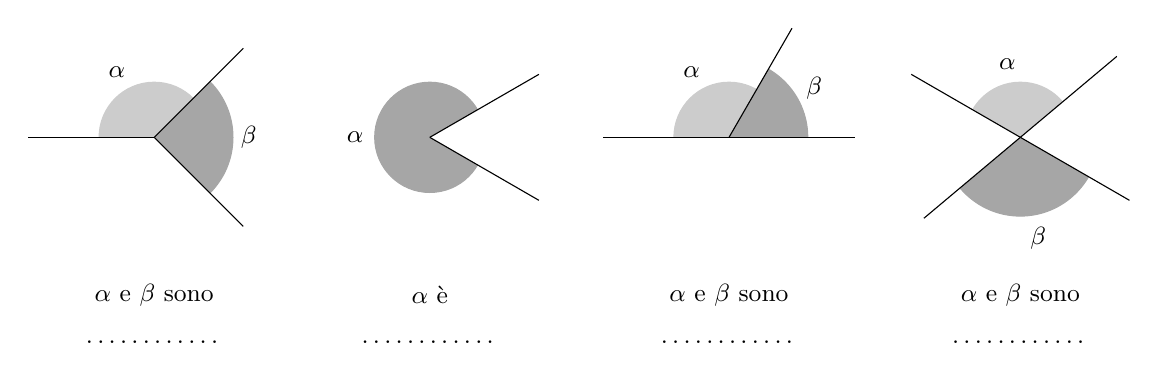
\begin{tikzpicture}
\pgfmathsetmacro{\myscale}{1};

\begin{scope}[scale={\myscale},font=\small]
\usetikzlibrary{calc}

\begin{scope}
\pgfmathsetmacro{\aalpha}{45};
\pgfmathsetmacro{\abeta}{180};
\pgfmathsetmacro{\agamma}{315};

\coordinate (o) at (0,0);
\coordinate (a) at ({\aalpha}:1.6);
\coordinate (b) at ({\abeta}:1.6);
\coordinate (c) at ({\agamma}:1.6);

\begin{scope}
\clip (o) -- (a) -- (-1,1) -- (b) -- cycle;
\draw[gray!40,fill=gray!40] circle[at=(o),radius=.7];
\end{scope}
\node at (120:0.95) {$\alpha$};

\begin{scope}
\clip (o) -- (a) -- (c) -- cycle;
\draw[gray!70,fill=gray!70] circle[at=(o),radius=1];
\end{scope}
\node at (0:1.2) {$\beta$};

\draw (o) -- (a);
\draw (o) -- (b);
\draw (o) -- (c);

\node at (0,-2) {$\alpha$ e $\beta$ sono};
\node at (0,-2.6) {\ldots\ldots\ldots\ldots};
\end{scope}

\begin{scope}[xshift=3.5cm]
\pgfmathsetmacro{\aalpha}{30};
\pgfmathsetmacro{\abeta}{330};

\coordinate (o) at (0,0);
\coordinate (a) at ({\aalpha}:1.6);
\coordinate (b) at ({\abeta}:1.6);

\begin{scope}
\clip (o) -- (a) -- (-1,1) -- (-1,-1) -- (b) -- cycle;
\draw[gray!70,fill=gray!70] circle[at=(o),radius=.7];
\end{scope}
\node at (180:0.95) {$\alpha$};

\draw (o) -- (a);
\draw (o) -- (b);

\node at (0,-2) {$\alpha$ \`e};
\node at (0,-2.6) {\ldots\ldots\ldots\ldots};
\end{scope}


\begin{scope}[xshift=7.3cm]
\pgfmathsetmacro{\aalpha}{60};
\pgfmathsetmacro{\abeta}{180};
\pgfmathsetmacro{\agamma}{360};

\coordinate (o) at (0,0);
\coordinate (a) at ({\aalpha}:1.6);
\coordinate (b) at ({\abeta}:1.6);
\coordinate (c) at ({\agamma}:1.6);

\begin{scope}
\clip (o) -- (a) -- (b) -- cycle;
\draw[gray!40,fill=gray!40] circle[at=(o),radius=.7];
\end{scope}
\node at (120:0.95) {$\alpha$};

\begin{scope}
\clip (o) -- (a) -- (c) -- cycle;
\draw[gray!70,fill=gray!70] circle[at=(o),radius=1];
\end{scope}
\node at (30:1.25) {$\beta$};

\draw (o) -- (a);
\draw (o) -- (b);
\draw (o) -- (c);

\node at (0,-2) {$\alpha$ e $\beta$ sono};
\node at (0,-2.6) {\ldots\ldots\ldots\ldots};
\end{scope}


\begin{scope}[xshift=11cm]
\pgfmathsetmacro{\aalpha}{40};
\pgfmathsetmacro{\abeta}{150};
\pgfmathsetmacro{\agamma}{220};
\pgfmathsetmacro{\adelta}{330};

\coordinate (o) at (0,0);
\coordinate (a) at ({\aalpha}:1.6);
\coordinate (b) at ({\abeta}:1.6);
\coordinate (c) at ({\agamma}:1.6);
\coordinate (d) at ({\adelta}:1.6);

\begin{scope}
\clip (o) -- (a) -- (b) -- cycle;
\draw[gray!40,fill=gray!40] circle[at=(o),radius=.7];
\end{scope}
\node at (100:0.95) {$\alpha$};

\begin{scope}
\clip (o) -- (c) -- (0,-1.3) -- (d) -- cycle;
\draw[gray!70,fill=gray!70] circle[at=(o),radius=1];
\end{scope}
\node at (280:1.3) {$\beta$};

\draw (o) -- (a);
\draw (o) -- (b);
\draw (o) -- (c);
\draw (o) -- (d);

\node at (0,-2) {$\alpha$ e $\beta$ sono};
\node at (0,-2.6) {\ldots\ldots\ldots\ldots};
\end{scope}

\end{scope}

\end{tikzpicture}

 \caption{Esercizio \ref{ese:1.57}}\label{fig:ese1.57}
\end{figure}
\end{inaccessibleblock}

\begin{esercizio}
\label{ese:1.58}
Rappresenta graficamente ciascuna delle seguenti situazioni:
\begin{enumeratea}
\item $A\widehat{O}B\cup A\widehat{O}C=A\widehat{O}B$;
\item $A\widehat{O}B\cap A\widehat{O}C=A\widehat{O}B$;
\item $A\widehat{O}B\cap 
C\widehat{O}D=C\widehat{O}B$~~e~~$A\widehat{O}B\cup 
C\widehat{O}D=A\widehat{O}B$.
\end{enumeratea}
\end{esercizio}

\begin{esercizio}
\label{ese:1.59}
Facendo riferimento alla figura~\ref{fig:ese1.59} indica
\begin{enumeratea}
\item una coppia di segmenti consecutivi \ldots\ldots\ldots\ldots{};
\item una coppia di segmenti adiacenti \ldots\ldots\ldots\ldots{};
\item una coppia di rette incidenti \ldots\ldots\ldots\ldots{};
\item una coppia di rette parallele \ldots\ldots\ldots\ldots{};
\item una coppia di angoli consecutivi \ldots\ldots\ldots\ldots{};
\item una coppia di angoli adiacenti \ldots\ldots\ldots\ldots{};
\item una coppia di angoli opposti al vertice 
\ldots\ldots\ldots\ldots{};
\item un angolo concavo \ldots\ldots\ldots\ldots{};
\item un angolo convesso \ldots\ldots\ldots\ldots{}
\end{enumeratea}
\end{esercizio}


\begin{inaccessibleblock}[Figura: TODO]
 \begin{figure}[htb]
 \centering% Copyright (c) 2015 Daniele Masini - d.masini.it@gmail.com

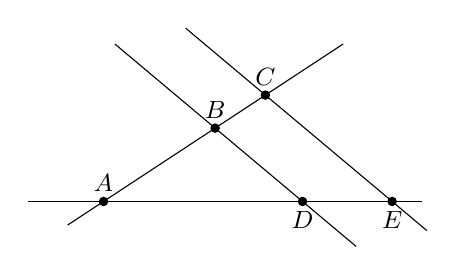
\begin{tikzpicture}[scale=1,font=\small]
\usetikzlibrary{calc}

\begin{scope}
\draw (0,0) coordinate (r1) -- (5,0) coordinate (r2);
\draw  (0.5,-.3) coordinate (s1) -- (4,2) coordinate (s2);
\draw  (1.1,2) coordinate (t1) -- +(-40:4) coordinate (t2);
\draw  (2,2.2) coordinate (u1) -- +(-40:4) coordinate (u2);
\coordinate (a) at (intersection of r1--r2 and s1--s2);
\coordinate (b) at (intersection of t1--t2 and s1--s2);
\coordinate (c) at (intersection of u1--u2 and s1--s2);
\coordinate (d) at (intersection of t1--t2 and r1--r2);
\coordinate (e) at (intersection of u1--u2 and r1--r2);
\draw[fill] (a) circle (1.5pt) node[above] {$A$};
\draw[fill] (b) circle (1.5pt) node[above] {$B$};
\draw[fill] (c) circle (1.5pt) node[above] {$C$};
\draw[fill] (d) circle (1.5pt) node[below] {$D$};
\draw[fill] (e) circle (1.5pt) node[below] {$E$};

\end{scope}


\end{tikzpicture}

 \caption{Esercizio \ref{ese:1.59}}\label{fig:ese1.59}
\end{figure}
\end{inaccessibleblock}

\begin{esercizio}
\label{ese:1.60}
Indica quali delle figure geometriche riportate nella 
figura~\ref{fig:ese1.60} sono convesse
\begin{multicols}{5}
\begin{enumeratea}
\item $A$, $B$, $C$, $G$;
\item $B$, $C$, $D$, $F$;
\item $B$, $C$, $D$;
\item $B$, $C$;
\item $D$, $E$, $F$, $G$.
\end{enumeratea}
\end{multicols}
\end{esercizio}


\begin{inaccessibleblock}[Figura: TODO]
 \begin{figure}[htb]
 \centering% Copyright (c) 2015 Daniele Masini - d.masini.it@gmail.com

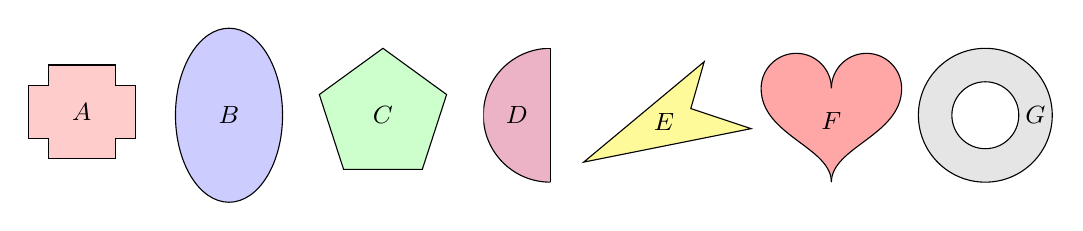
\begin{tikzpicture}[scale=0.85,font=\small]
\usetikzlibrary{calc}

\begin{scope}[yshift=.75cm]
\draw[fill=pink!80] (0,0) -- (1,0) -- (1,-.3) -- (1.3,-.3) -- (1.3,-1.1) -- (1,-1.1) -- (1,-1.4) -- (0,-1.4) -- (0,-1.1) -- (-.3,-1.1) -- (-.3,-.3) -- (0,-.3) -- cycle;
\node at (.5,-.7) {$A$};
\end{scope}

\begin{scope}[xshift=2.7cm]
\draw[fill=blue!20] (0,0) circle [x radius=.8cm, y radius=1.3cm];
\node at (0,0) {$B$};
\end{scope}

\begin{scope}[xshift=5cm,rotate=18]
\coordinate (o) at (0,0);
\coordinate (p0) at (0:1cm);
\coordinate (p1) at (1*72:1cm);
\coordinate (p2) at (2*72:1cm);
\coordinate (p3) at (3*72:1cm);
\coordinate (p4) at (4*72:1cm);
\draw[fill=green!20] (p0) -- (p1) -- (p2) -- (p3) -- (p4) -- cycle;
\node at (o) {$C$};
\end{scope}

\begin{scope}[xshift=7.5cm]
\begin{scope}
\clip (-1,-1.1) rectangle (0,1);
\draw[fill=purple!30] (0,0) circle (1cm);
\end{scope}
\draw (0,-1) -- (0,1);
\node at (-0.5,0) {$D$};
\end{scope}

\begin{scope}[xshift=8cm,yshift=-0.7cm]
\draw[fill=yellow!40] (0,0) -- (2.5,0.5) -- (1.6,0.8) -- (1.8,1.5) -- cycle;
\node at (1.2,0.6) {$E$};
\end{scope}

\begin{scope}[xshift=11.7cm,yshift=-1cm,scale=.7]
\draw[fill=red!35] (0,0) .. controls (0,0.75) and (-1.5,1) .. (-1.5,2)  arc (180:0:0.75);
\draw[red!35] (0,0) -- (0,2);
\draw[fill=red!35] (0,0) .. controls (0,0.75) and ( 1.5,1) .. ( 1.5,2)  arc (0:180:0.75);
\node at (0,1.3) {$F$};
\end{scope}

\begin{scope}[xshift=14cm]
\draw[fill=gray!20] (0,0) circle (1cm);
\begin{scope}
\clip (0,0) circle (1cm);
\draw[fill,white] (0,0) circle (.5cm);
\end{scope}
\draw (0,0) circle (.5cm);
\node at (0.75,0) {$G$};
\end{scope}

\end{tikzpicture}

 \caption{Esercizio~\ref{ese:1.60}}\label{fig:ese1.60}
\end{figure}
\end{inaccessibleblock}

\begin{esercizio}
\label{ese:1.61}
Scrivi per esteso nel linguaggio comune quanto è indicato in simboli 
e rappresenta con un disegno tutti i casi possibili: $(P\in r)\wedge 
(P\in s)\wedge (Q\in r)$.
\end{esercizio}

\begin{esercizio}
\label{ese:1.62}
Descrivi la costruzione della figura~\ref{fig:ese1.62}, dove le rette 
$c$ e $d$ sono parallele.
\end{esercizio}


\begin{inaccessibleblock}[Figura: TODO]
 \begin{figure}[htb]
 \centering% Copyright (c) 2015 Daniele Masini - d.masini.it@gmail.com

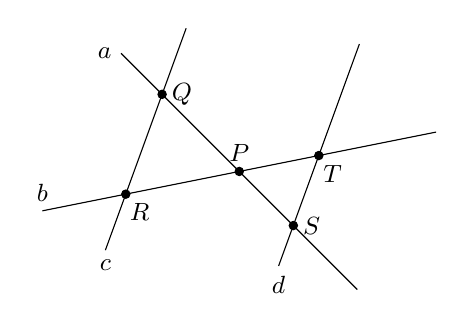
\begin{tikzpicture}[scale=1,font=\small]
\usetikzlibrary{calc}

\begin{scope}
\draw (0,0) node[above] {$b$} coordinate (b1) -- (5,1) coordinate (b2);
\draw (1,2) node[left] {$a$} coordinate (a1) -- (4,-1) coordinate (a2);
\draw (0.8,-0.5) node[below] {$c$} coordinate (c1) -- +(70:3) coordinate (c2);
\draw (3,-0.7) node[below] {$d$} coordinate (d1) -- +(70:3) coordinate (d2);

\coordinate (p) at (intersection of b1--b2 and a1--a2);
\draw[fill] (p) circle (1.5pt) node[above] {$P$}; 
\coordinate (q) at (intersection of a1--a2 and c1--c2);
\draw[fill] (q) circle (1.5pt) node[right] {$Q$}; 
\coordinate (r) at (intersection of b1--b2 and c1--c2);
\draw[fill] (r) circle (1.5pt) node[right=5pt, below] {$R$}; 
\coordinate (s) at (intersection of a1--a2 and d1--d2);
\draw[fill] (s) circle (1.5pt) node[right] {$S$}; 
\coordinate (t) at (intersection of b1--b2 and d1--d2);
\draw[fill] (t) circle (1.5pt) node[right=5pt, below] {$T$}; 

\end{scope}

\end{tikzpicture}

 \caption{Esercizio~\ref{ese:1.62}}\label{fig:ese1.62}
\end{figure}
\end{inaccessibleblock}
 
\begin{esercizio}
\label{ese:1.63}
Se $P$ è centro di un fascio di rette e $A$ è un punto dello stesso 
piano, è vero che nel fascio di centro $P$ esiste una retta passante 
per $A$?
\end{esercizio}

\begin{esercizio}
\label{ese:1.64}
Motiva la verità o la falsità della proposizione: <<Tutte le rette 
incidenti formano 2 coppie di angoli opposti al vertice>>.
\end{esercizio}

\begin{esercizio}
\label{ese:1.65}
Siano $a$, $b$, $c$, $d$ quattro semirette aventi l'origine in comune 
$O$ disposte in ordine antiorario come nella 
figura~\ref{fig:ese1.65}. Individua, aiutandoti con il disegno, quali 
sono gli angoli che si ottengono dalle seguenti operazioni:
\begin{multicols}{3}
\begin{enumeratea}
\item $a\widehat{O}d \cap d\widehat{O}b$;
\item $d\widehat{O}c \cup c\widehat{O}b$;
\item $c\widehat{O}b \cup c\widehat{O}a$;
\item $a\widehat{O}b \cap d\widehat{O}b$;
\item $c\widehat{O}a \cap d\widehat{O}b$.
\end{enumeratea}
\end{multicols}
\end{esercizio}


\begin{inaccessibleblock}[Figura: TODO]
 \begin{figure}[htb]
 \centering% Copyright (c) 2015 Daniele Masini - d.masini.it@gmail.com

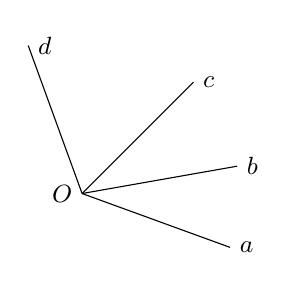
\begin{tikzpicture}[scale=1,font=\small]
\usetikzlibrary{calc}

\begin{scope}
\pgfmathsetmacro{\aalpha}{-20};
\pgfmathsetmacro{\abeta}{10};
\pgfmathsetmacro{\agamma}{45};
\pgfmathsetmacro{\adelta}{110};

\draw (0,0) coordinate (o) node[left] {$O$} -- +({\aalpha}:2) node[right] {$a$};
\draw (o) -- +({\abeta}:2) node[right] {$b$};
\draw (o) -- +({\agamma}:2) node[right] {$c$};
\draw (o) -- +({\adelta}:2) node[right] {$d$};
\end{scope}

\end{tikzpicture}

 \caption{Esercizio~\ref{ese:1.65}}\label{fig:ese1.65}
\end{figure}
\end{inaccessibleblock}

\begingroup
\hypersetup{linkcolor=black}
\subsubsection*{\ref{sect:operazioni_segmenti_angoli} - 
\nameref{sect:operazioni_segmenti_angoli}}
\endgroup

\begin{esercizio}
\label{ese:1.66}
Due angoli sono complementari e uno è doppio dell'altro. Quale delle 
seguenti affermazioni è vera?
\begin{enumeratea}
\item uno è retto e l'altro è piatto;
\item uno è $1/3$ dell'angolo retto e l'altro i $2/3$ dell'angolo 
retto;
\item uno è $1/3$ dell'angolo retto e l'altro $1/6$ dell'angolo retto;
\item uno è $1/2$ dell'angolo retto e l'altro è retto;
\item uno è $2/3$ dell'angolo retto e l'altro i $4/6$ dell'angolo 
retto.
\end{enumeratea}
\end{esercizio}

\begin{esercizio}
\label{ese:1.67}
Siano $\alpha$ e $\beta$ due angoli consecutivi esplementari e siano 
$a$ e $b$ le loro bisettrici. L'angolo tra $a$ e $b$ è
\begin{multicols}{2}
\begin{enumeratea}
\item piatto;
\item retto;
\item nullo;
\item non si può sapere.
\end{enumeratea}
\end{multicols}
\end{esercizio}

\begin{esercizio}
\label{ese:1.68}
Se $\alpha$ e $\beta$ sono due angoli di vertice $O$, consecutivi e 
complementari e $a$ e $b$ le loro bisettrici, allora dell'angolo 
$a\widehat{O}b$ si può dire  che:
\begin{multicols}{2}
\begin{enumeratea}
\item è uguale all'angolo retto;
\item è la metà di un angolo retto;
\item è la terza parte di un angolo retto;
\item è la quarta parte di un angolo retto;
\item non è possibile determinarne l'ampiezza.
\end{enumeratea}
\end{multicols}
\end{esercizio}

\begin{esercizio}
\label{ese:1.69}
Le bisettrici di due angoli adiacenti:
\begin{multicols}{2}
\begin{enumeratea}
\item sono parallele;
\item sono lati di un angolo retto;
\item sono lati di un angolo concavo;
\item coincidono;
\item sono semirette opposte.
\end{enumeratea}
\end{multicols}
\end{esercizio}

\begin{esercizio}
\label{ese:1.70}
Due angoli si dicono complementari quando:
\begin{multicols}{2}
\begin{enumeratea}
\item sono consecutivi;
\item sono angoli opposti al vertice;
\item la loro somma è un angolo retto;
\item ciascuno di essi è acuto;
\item ciascuno è la metà di un angolo retto.
\end{enumeratea}
\end{multicols}
\end{esercizio}

\begin{esercizio}
\label{ese:1.71}
Dati due segmenti adiacenti $AB$ e $BC$ tali che $AB\cong 
\frac{1}{3}\cdot BC$, allora per $AC=AB+BC$ si può dire che:
\begin{multicols}{3}
\begin{enumeratea}
\item $AC\cong \frac{1}{4}\cdot BC$;
\item $AC\cong 3\cdot BC$;
\item $AC\cong 2\cdot BC$;
\item $AC\cong \frac{1}{2}\cdot BC$;
\item $AC\cong \frac{4}{3}\cdot BC$.
\end{enumeratea}
\end{multicols}
\end{esercizio}

\begin{esercizio}
\label{ese:1.72}
Due segmenti $AB$ e $CD$ appartengono alla stessa retta e hanno lo 
stesso punto medio. Si può affermare che:
\begin{multicols}{5}
\begin{enumeratea}
\item $AB\cong CD$;
\item $AC\cong CD$;
\item $DB\cong DC$;
\item $AC\cong BD$;
\item $AC\cong AB$.
\end{enumeratea}
\end{multicols}
\end{esercizio}

\begin{esercizio}
\label{ese:1.73}
Per ciascuna delle affermazioni seguenti, dire se è vera o falsa, e 
spiegare perché
\begin{enumeratea}
\item l'angolo retto è la metà dell'angolo giro	
\tab\tab\tab\qquad\boxV\quad\boxF
\item ogni angolo convesso ha due bisettrici		
\tab\tab\tab\qquad\boxV\quad\boxF
\item due angoli che hanno in comune il vertice sono 
consecutivi	\tab\qquad\boxV\quad\boxF
\item un angolo ottuso è maggiore di qualunque angolo acuto	
	\tab\qquad\boxV\quad\boxF
\item sommando due angoli acuti si può ottenere un angolo 
piatto	\tab\qquad\boxV\quad\boxF
\end{enumeratea}
\end{esercizio}

\begin{esercizio}
\label{ese:1.74}
Tre semirette $a$, $b$, $c$ uscenti da uno stesso punto dividono il 
piano in tre angoli congruenti. Dopo aver rappresentato le semirette, 
traccia la semiretta $b_1$ opposta di $b$. Quale delle seguenti 
affermazioni è vera?
\begin{enumeratea}
\item $b_1$ è perpendicolare alla semiretta $a$;
\item $b_1$ è bisettrice dell'angolo formato da $a$ e $c$;
\item $b_1$ è perpendicolare alla semiretta $c$;
\end{enumeratea}
\end{esercizio}

\begin{esercizio}
\label{ese:1.75}
Dato l'angolo acuto $A\widehat{O}B$, sia $OC$ la sua bisettrice. Sia 
poi $OD$ una semiretta esterna all'angolo come nella 
figura~\ref{fig:ese1.75}, quale relazione è vera?
\begin{multicols}{2}
\begin{enumeratea}
\item $C\widehat{O}B\cong 
\frac{1}{2}\cdot(D\widehat{O}A-D\widehat{O}B)$;
\item $C\widehat{O}B\cong (A\widehat{O}D-A\widehat{O}B)$;
\item $C\widehat{O}B\cong (B\widehat{O}D-C\widehat{O}B)$;
\item $C\widehat{O}B\cong 
\frac{1}{2}\cdot(D\widehat{O}A+D\widehat{O}B)$.
\end{enumeratea}
\end{multicols}
\end{esercizio}


\begin{inaccessibleblock}[Figura: TODO]
 \begin{figure}[htb]
 \centering% Copyright (c) 2015 Daniele Masini - d.masini.it@gmail.com

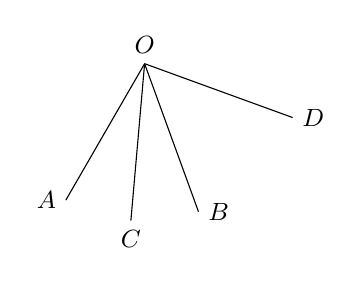
\begin{tikzpicture}[scale=1,font=\small]
\usetikzlibrary{calc}

\begin{scope}
\pgfmathsetmacro{\aalpha}{240};
\pgfmathsetmacro{\abeta}{290};
\pgfmathsetmacro{\agamma}{265};
\pgfmathsetmacro{\adelta}{340};

\draw (0,0) coordinate (o) node[above] {$O$} -- +({\aalpha}:2) node[left] {$A$};
\draw (o) -- +({\abeta}:2) node[right] {$B$};
\draw (o) -- +({\agamma}:2) node[below] {$C$};
\draw (o) -- +({\adelta}:2) node[right] {$D$};
\end{scope}

\end{tikzpicture}

 \caption{Esercizio~\ref{ese:1.75}}\label{fig:ese1.75}
\end{figure}
\end{inaccessibleblock}

\begin{esercizio}
\label{ese:1.76}
Individua tra gli angoli rappresentati nella figura~\ref{fig:ese1.76} 
quello piatto, quello retto, quello acuto, quello ottuso e quello 
concavo, scrivendolo nelle relative etichette. Per ciascuno di essi 
traccia la bisettrice.
\end{esercizio}


\begin{inaccessibleblock}[Figura: TODO]
 \begin{figure}[htb]
 \centering% Copyright (c) 2015 Daniele Masini - d.masini.it@gmail.com

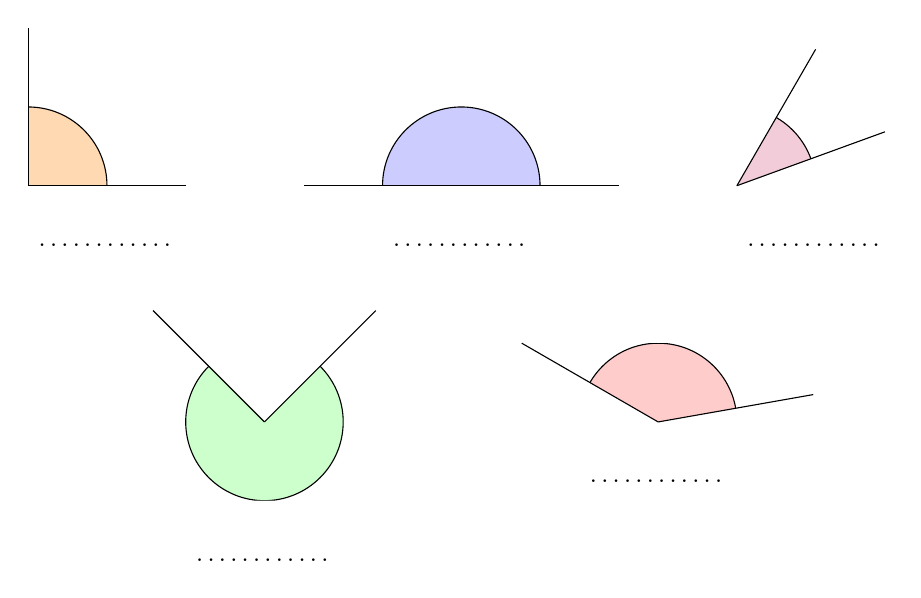
\begin{tikzpicture}[scale=1,font=\small]
\usetikzlibrary{calc}

\begin{scope}[xshift=-1.5cm]
\pgfmathsetmacro{\aalpha}{0};
\pgfmathsetmacro{\abeta}{90};
\coordinate (o) at (0,0);
\begin{scope}
\clip (o) rectangle (1.5,1.5);
\draw[fill=orange!30] (o) circle (1cm);
\end{scope}
\draw (o) -- +({\aalpha}:2);
\draw (o) -- +({\abeta}:2);
\node at (1,-.75) {\ldots\ldots\ldots\ldots};
\end{scope}

\begin{scope}[xshift=4cm]
\pgfmathsetmacro{\aalpha}{0};
\pgfmathsetmacro{\abeta}{180};
\coordinate (o) at (0,0);
\begin{scope}
\clip (-1.5,0) rectangle (1.5,1.5);
\draw[fill=blue!20] (o) circle (1cm);
\end{scope}
\draw (o) -- +({\aalpha}:2);
\draw (o) -- +({\abeta}:2);
\node at (0,-.75) {\ldots\ldots\ldots\ldots};
\end{scope}

\begin{scope}[xshift=7.5cm]
\pgfmathsetmacro{\aalpha}{20};
\pgfmathsetmacro{\abeta}{60};
\coordinate (o) at (0,0);
\begin{scope}
\clip (o) -- ({\aalpha}:1.5) -- ({\abeta}:1.5) -- cycle;
\draw[fill=purple!20] (o) circle (1cm);
\end{scope}
\draw (o) -- +({\aalpha}:2);
\draw (o) -- +({\abeta}:2);
\node at (1,-.75) {\ldots\ldots\ldots\ldots};
\end{scope}

\begin{scope}[xshift=1.5cm, yshift=-3cm]
\pgfmathsetmacro{\aalpha}{135};
\pgfmathsetmacro{\abeta}{405};
\coordinate (o) at (0,0);
\begin{scope}
\clip (o) -- ({\aalpha}:1.5) -- (-1.5,0) -- (-1.5,-1) -- (1.5,-1) -- (1.5,0) -- ({\abeta}:1.5) -- cycle;
\draw[fill=green!20] (o) circle (1cm);
\end{scope}
\draw (o) -- +({\aalpha}:2);
\draw (o) -- +({\abeta}:2);
\node at (0,-1.75) {\ldots\ldots\ldots\ldots};
\end{scope}

\begin{scope}[xshift=6.5cm, yshift=-3cm]
\pgfmathsetmacro{\aalpha}{10};
\pgfmathsetmacro{\abeta}{150};
\coordinate (o) at (0,0);
\begin{scope}
\clip (o) -- ({\aalpha}:1.5) -- (1.5,1) -- (-1.5,1) -- ({\abeta}:1.5) -- cycle;
\draw[fill=red!20] (o) circle (1cm);
\end{scope}
\draw (o) -- +({\aalpha}:2);
\draw (o) -- +({\abeta}:2);
\node at (0,-0.75) {\ldots\ldots\ldots\ldots};
\end{scope}

\end{tikzpicture}

 \caption{Esercizio~\ref{ese:1.76}}\label{fig:ese1.76}
\end{figure}
\end{inaccessibleblock}

\begin{esercizio}
\label{ese:1.77}
Per ognuna delle seguenti affermazioni indica se è vera oppure falsa
\begin{enumeratea}
\item Sommando due angoli acuti si ottiene sempre un angolo 
acuto		\hfill\boxV\quad\boxF
\item Sommando due angoli piatti si ottiene un angolo giro	
			\hfill\boxV\quad\boxF
\item Sommando un angolo acuto e uno retto si ottiene un angolo 
ottuso	\hfill\boxV\quad\boxF
\item Sommando due angoli retti si ottiene un angolo giro	
			\hfill\boxV\quad\boxF
\item Sommando un angolo piatto e un angolo acuto si ottiene un 
angolo concavo	\hfill\boxV\quad\boxF
\item Sommando due angoli convessi si ottiene sempre un angolo 
convesso	\hfill\boxV\quad\boxF
\item Sommando un angolo retto e un angolo piatto si ottiene un 
angolo giro		\hfill\boxV\quad\boxF
\end{enumeratea}
\end{esercizio}

\begin{esercizio}
\label{ese:1.78}
Individua l'angolo
\begin{enumeratea}
\item La differenza tra un angolo piatto è un angolo retto è un 
angolo \ldots\ldots\ldots\ldots\ldots\ldots{}
\item La differenza tra un angolo giro e un angolo piatto è un angolo 
\ldots\ldots\ldots\ldots\ldots\ldots{}
\item La differenza tra un angolo acuto e un angolo retto è un angolo 
\ldots\ldots\ldots\ldots\ldots\ldots{}
\item La differenza tra un angolo giro e un angolo piatto è un angolo 
\ldots\ldots\ldots\ldots\ldots\ldots{}
\item Il doppio di un angolo piatto è un angolo 
\ldots\ldots\ldots\ldots\ldots\ldots{}
\item Il doppio di un angolo retto è un angolo 
\ldots\ldots\ldots\ldots\ldots\ldots{}
\end{enumeratea}
\end{esercizio}
	
\begin{esercizio}
\label{ese:1.79}
Spiega perché se due angoli sono complementari i loro doppi sono 
supplementari.
\end{esercizio}

\begin{esercizio}
\label{ese:1.80}
Verifica, aiutandoti con un disegno, che se $\widehat{A}\cong 
\widehat{B}$ e $\widehat{C}<\widehat{D}$ allora 
$\widehat{A}+\widehat{C}<\widehat{B}+\widehat{D}$.
\end{esercizio}

\begin{esercizio}
\label{ese:1.81}
Un angolo $\alpha$ è retto e un angolo $\beta$ è la sesta parte di un 
angolo piatto. A quale frazione di angolo retto corrisponde la somma 
$\alpha + \beta$?
\end{esercizio}

\begin{esercizio}
\label{ese:1.82}
Dati quattro segmenti $AB>BC>CD>DE$. Verifica, aiutandoti con dei 
disegni, che:
\begin{multicols}{2}
\begin{enumeratea}
\item $AB-CD > BC-CD$;
\item $AB+DE > BC+CD$.
\end{enumeratea}
\end{multicols}
\end{esercizio}

\begin{esercizio}
\label{ese:1.83}
Disegna due angoli consecutivi $\alpha$ e $\beta$, disegna l'angolo 
$\gamma$ adiacente ad $\alpha$ non contenente $\beta$ e l'angolo 
$\delta$ adiacente a $\beta$ non contenente $\alpha$. Gli angoli 
$\gamma + \delta$ e $\alpha+\beta$ sono:
\begin{multicols}{2}
\begin{enumeratea}
\item complementari;
\item supplementari;
\item opposti al vertice;
\item esplementari.
\end{enumeratea}
\end{multicols}
\end{esercizio}

\begin{multicols}{2}
 
\begin{esercizio}
\label{ese:1.84}
Su una semiretta di origine $A$ segna il segmento $AB$, il segmento 
$BC\cong 3\cdot AB$ e il segmento $CD\cong AB$, i punti sono 
consecutivi secondo l'ordine alfabetico. Secondo quale numero 
frazionario $AD$ è multiplo di $BC$?
\end{esercizio}

\begin{esercizio}
\label{ese:1.85}
Su una semiretta di origine $O$ si hanno i segmenti $OA$ e $OB$ con 
$OB>OA$. Se $M$ è il punto medio di $OA$ e $N$ è il punto medio di 
$OB$, quale delle due seguenti relazioni è vera?
\begin{enumeratea}
\item $MN\cong \frac{1}{2}\cdot(OB-OA)$;
\item $MN\cong \frac{1}{2}\cdot(OB+OA)$.
\end{enumeratea}
\end{esercizio}

\begin{esercizio}
\label{ese:1.86}
Su una semiretta di origine $O$ si prendono i punti $A$, $B$ e $C$ 
con $OC>OB>OA$. Sia $M$ il punto medio di $OA$ e $N$ il punto medio 
di $BC$. Quale delle seguenti relazioni è vera?
\begin{enumeratea}
\item $MN\cong\frac{1}{2}\cdot(OB+OA)$;
\item $MN\cong\frac{1}{2}\cdot(OA+BC)$;
\item $MN\cong\frac{1}{2}\cdot(OC+AB)$.
\end{enumeratea}
\end{esercizio}

\begin{esercizio}
\label{ese:1.87}
Su una retta, i punti $A$, $B$, $C$, $D$ si susseguono secondo 
l'ordine alfabetico. Se $AB$ è congruente a $CD$ i punti medi di $BC$ 
e $AD$ coincidono? Spiega perché?
\end{esercizio}

\begin{esercizio}
\label{ese:1.88}
Siano $AB$ e $CD$ due segmenti congruenti disposti su una retta $r$ e 
non aventi alcun punto in comune. Dimostra che $AC$ è congruente a 
$BD$.
\end{esercizio}

\begin{esercizio}
\label{ese:1.89}
Siano $AB$ e $CD$ due segmenti congruenti disposti su una retta $r$, 
non aventi alcun punto in comune e in modo che $AB$ preceda $CD$. 
Dimostra che il punto medio di $BC$ è anche punto medio di $AD$.
\end{esercizio}

\begin{esercizio}
\label{ese:1.90}
Siano $AB$ e $CD$ due segmenti congruenti adiacenti, siano $M$ e $N$ 
i rispettivi punti medi, dimostra che $MN$ è congruente a $CD$.
\end{esercizio}

\begin{esercizio}
\label{ese:1.91}
Siano $AB$ e $CD$ due segmenti congruenti adiacenti tali che $BC\cong 
3\cdot AB$, siano $M$ e $N$ i rispettivi punti medi, dimostra che 
$MN\cong \frac{2}{3}\cdot BC$.
\end{esercizio}

\begin{esercizio}
\label{ese:1.92}
Siano $AB$ e $BC$ due segmenti adiacenti non necessariamente 
congruenti, sia $M$ il punto medio di $AC$ ed $N$ il punto medio di 
$BC$, dimostra che $MN\cong \frac{1}{2}\cdot AB$.
\end{esercizio}

\begin{esercizio}
\label{ese:1.93}
Dati due segmenti adiacenti $AB$ e $BC$ e $M$ e $N$ i loro rispettivi 
punti medi, dimostrare che $AB\cong MN$.
\end{esercizio}

\begin{esercizio}
\label{ese:1.94}
Siano $AB$ e $BC$ due segmenti adiacenti e siano $M$ e $N$ i loro 
rispettivi punti medi. Dimostrare che se~~$AB < BC$~~allora~~$AB < MN 
< BC$.
\end{esercizio}
 
\begin{esercizio}
\label{ese:1.95}
In un piano gli angoli $A\widehat{O}C$ e $C\widehat{O}D$ sono 
adiacenti. Sia $OF$ la bisettrice di $A\widehat{O}C$ e $OE$ la 
bisettrice di $C\widehat{O}D$. Spiega perché $F\widehat{O}E$ è retto.
\end{esercizio}

\begin{esercizio}
\label{ese:1.96}
Quattro semirette con origine nello stesso punto dividono un angolo 
giro in quattro angoli $\alpha$, $\beta$, $\gamma$, $\delta$ disposti 
in senso antiorario secondo l'ordine alfabetico. Si sa che $\alpha$ è 
congruente a $\gamma$ e $\beta$ è congruente a $\delta$. Dimostra che 
ci sono alcune semirette opposte, quali sono?
\end{esercizio}

\begin{esercizio}
\label{ese:1.97}
Disegna un angolo convesso e i suoi complementari consecutivi, spiega 
come hai costruito gli angoli complementari. Spiega perché i 
complementari dello stesso angolo sono congruenti.
\end{esercizio}

\begin{esercizio}
\label{ese:1.98}
Sia $M$ il punto medio del segmento $AB$ e sia $P$ un punto compreso 
tra $M$ e $B$. Che relazione esiste tra $MP$ e la differenza $AP-BP$? 
\emph{Per aiutarti costruisci il punto $Q$ tale che $QM\cong MP$.}
\end{esercizio}

\begin{esercizio}
\label{ese:1.99}
Sia $A\widehat{O}B$ un angolo qualunque e $OC$ la sua bisettrice. Sia 
$OD$ una semiretta esterna all'angolo $A\widehat{O}B$. Che relazione 
c'è tra $C\widehat{O}D$ e $A\widehat{O}D+B\widehat{O}D$? \emph{Per 
aiutarti traccia la bisettrice di $B\widehat{O}D$.}
\end{esercizio}

\begin{esercizio}
\label{ese:1.100}
Dimostrare che le bisettrici di due angoli adiacenti formano un 
angolo retto.
\end{esercizio}

\begin{esercizio}
\label{ese:1.101}
Due rette incidenti formano quattro angoli, dimostra che le 
bisettrici degli angoli sono tra loro perpendicolari.
\end{esercizio}

\begin{esercizio}
\label{ese:1.102}
Siano $a\widehat{O}b$ e $b\widehat{O}c$ due angoli convessi 
consecutivi, siano $d$ ed $e$ le loro rispettive bisettrici. Dimostra 
che $a\widehat{O}c\cong 2\cdot d\widehat{O}e$.
\end{esercizio}

\begin{esercizio}
\label{ese:1.103}
Dati due angoli consecutivi $a\widehat{O}b$ e $b\widehat{O}c$, e le 
loro rispettive bisettrici $d$ ed $e$, dimostra che se 
$d\widehat{O}b$ e $b\widehat{O}e$ sono complementari allora gli 
angoli $a\widehat{O}b$ e $b\widehat{O}c$ sono adiacenti. Dimostra 
anche che se $a\widehat{O}b$ e $b\widehat{O}c$ sono adiacenti allora  
$d\widehat{O}b$ e $b\widehat{O}e$ sono complementari.
\end{esercizio}

\begingroup
\hypersetup{linkcolor=black}
\subsubsection*{\ref{sect:misura} - \nameref{sect:misura}}
\endgroup

\begin{esercizio}
\label{ese:1.104}
Due segmenti adiacenti $AB$ e $BC$ misurano rispettivamente 12~cm e 
15~cm, calcola la misura della distanza tra i loro punti medi $M$ e 
$N$.
\end{esercizio}

\begin{esercizio}
\label{ese:1.105}
Dati due segmenti $AB$ e $CD$, con $\overline{AB} = 5$~cm e 
$\overline{CD} = 6$~cm, sottrai dalla loro somma la loro differenza e 
verifica che si ottiene un segmento congruente al doppio del segmento 
minore.
\end{esercizio}

\begin{esercizio}
\label{ese:1.106}
Il triplo di un segmento $AB$ uguaglia il quadruplo di un segmento 
$CD$; determinare il rapporto tra $AB$ e $CD$.
\end{esercizio}

\begin{esercizio}
\label{ese:1.107}
Due segmenti $AP$ e $PB$ sono tali che $\frac{AP}{PB}=\frac{4}{7}$; 
determina la misura del segmento $AB=AP+PB$, sapendo che $AP$ misura 
16~cm.
\end{esercizio}

\begin{esercizio}
\label{ese:1.108}
I segmenti $OA$, $AB$ e $BC$ sono adiacenti; $M$ ed $N$ sono 
rispettivamente i punti medi di $OA$ e di $BC$. Se 
$\overline{OA}=4$~m, $\overline{AB}=7$~m e $\overline{MN}=14$~m, 
quanto misura $BC$?
\end{esercizio}

\begin{esercizio}
\label{ese:1.109}
Su una semiretta di origine $O$ sono disposti tre punti $A$, $B$, $C$ 
tali che $\overline{OB}=4\overline{AB}$, $\overline{OB}=16$~cm, $BC$ 
supera $AB$ di 2~cm. Determina la lunghezza di $BC$.
\end{esercizio}

\begin{esercizio}
\label{ese:1.110}
Calcola la misura dell'ampiezza di due angoli di cui si sa che sono 
complementari e che la loro differenza misura $12\grado30'$.
\end{esercizio}
 
\begin{esercizio}
\label{ese:1.111}
Calcola la misura di due angoli adiacenti, di cui si sa che uno è 
$3/4$ dell'altro.
\end{esercizio}

\begin{esercizio}
\label{ese:1.112}
Un angolo che sia i $3/5$ di un angolo giro misura
\begin{multicols}{2}
\begin{enumeratea}
\item $72\grado$;	\item $216\grado$;	\item 
$330\grado$;	\item $550\grado$.
\end{enumeratea}
\end{multicols}
\end{esercizio}

\begin{esercizio}
\label{ese:1.113}
Se ad un angolo retto sommo i suoi $5/3$ ottengo un angolo la cui 
misura è
\begin{multicols}{2}
\begin{enumeratea}
\item $240\grado$;	\item $150\grado$;	\item 
$144\grado$;	\item $125\grado$.
\end{enumeratea}
\end{multicols}
\end{esercizio}
	
\begin{esercizio}
\label{ese:1.114}
Le quattro semirette $a$, $b$, $c$, $d$ hanno la stessa origine $O$ e 
sono disposte in senso antiorario; $m$ è la bisettrice sia 
dell'angolo $a\widehat{O}d$ che dell'angolo $b\widehat{O}c$. Sapendo 
che $b\widehat{O}c$ misura $70\grado$ e che $a\widehat{O}d$ misura 
$110\grado$, quanto misurano gli angoli $a\widehat{O}b$ e 
$c\widehat{O}d$?
\end{esercizio}

\begin{esercizio}
\label{ese:1.115}
La somma di due angoli è $3/4$ di un angolo retto. Sapendo che uno è 
doppio dell'altro quale frazione di angolo retto è ciascuno dei due 
angoli?
\end{esercizio}

\begin{esercizio}
\label{ese:1.116}
Disegna tre angoli consecutivi $a\widehat{O}b$, $b\widehat{O}c$ e 
$c\widehat{O}d$ di cui si sa che la loro somma è un angolo piatto e 
che $a\widehat{O}b$ è $2/3$ dell'angolo piatto. Determina quanto 
misura l'angolo formato dalle bisettrici degli angoli $b\widehat{O}c$ 
e $c\widehat{O}d$.
\end{esercizio}

\begin{esercizio}
\label{ese:1.117}
Di due angoli adiacenti uno è i sette terzi dell'altro; calcola 
l'ampiezza di ciascun angolo.
\end{esercizio}

\begin{esercizio}
\label{ese:1.118}
La somma di tre angoli misura $200\grado$; sapendo che il primo è 
cinque terzi del secondo e questo è tre quarti del terzo, trovare 
l'ampiezza di ognuno.
\end{esercizio}

\begin{esercizio}
\label{ese:1.119}
La somma di tre angoli consecutivi è un angolo giro. Sapendo che il 
primo è due terzi del secondo e questo è tre quarti del terzo, qual è 
l'ampiezza di ogni angolo?
\end{esercizio}

\begin{esercizio}
\label{ese:1.120}
Determinare la misura dei due segmenti $AB$ e $CD$ sapendo che 
$AB\cong \frac{5}{7}\cdot CD$ e che la loro somma è 24~cm.
\end{esercizio}

\begin{esercizio}
\label{ese:1.121}
Determinare la misura di due segmenti sapendo che il loro rapporto è 
$5/7$ e la loro differenza è 12~cm.
\end{esercizio}

\begin{esercizio}
\label{ese:1.122}
La somma di due segmenti è 21~cm e il minore di essi supera di 5~cm i 
$3/4$ del maggiore. Calcola la misura di ciascun segmento.
\end{esercizio}

\begin{esercizio}
\label{ese:1.123}
Determina la lunghezza di due segmenti sapendo che l'uno supera 
l'altro di 12~cm e che la loro somma è 102~cm.
\end{esercizio}

\begin{esercizio}
\label{ese:1.124}
Un segmento, lungo 59~cm, è stato diviso in parti. Sapendo che i 
$5/6$ di una parte sono uguali ai quattro settimi dell'altra, qual è 
la lunghezza di ogni parte?
\end{esercizio}

\end{multicols}

\begingroup
\hypersetup{linkcolor=black}
\subsubsection*{\ref{sect:poligoni} - \nameref{sect:poligoni}}
\endgroup

\begin{esercizio}
\label{ese:1.125}
Quante diagonali ha un triangolo?
\begin{multicols}{4}
\begin{enumeratea}
\item nessuna;
\item 1;
\item 2;
\item 3.
\end{enumeratea}
\end{multicols}
\end{esercizio}

\begin{esercizio}
\label{ese:1.126}
Quante diagonali puoi tracciare dal vertice di un poligono di 6 lati?
\begin{multicols}{4}
\begin{enumeratea}
\item 6;
\item 5;
\item 4;
\item 3.
\end{enumeratea}
\end{multicols}
\end{esercizio}

\begin{esercizio}
\label{ese:1.127}
Traccia l'angolo esterno relativo agli angoli interni indicati con un 
arco nella figura~\ref{fig:ese1.127}.
\end{esercizio}


\begin{inaccessibleblock}[Figura: TODO]
 \begin{figure}[htb]
 \centering% Copyright (c) 2015 Daniele Masini - d.masini.it@gmail.com

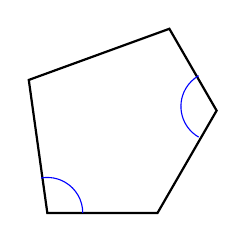
\begin{tikzpicture}[scale=1,font=\small]
\usetikzlibrary{calc}

\begin{scope}
\pgfmathsetmacro{\aalpha}{60};
\pgfmathsetmacro{\abeta}{120};
\pgfmathsetmacro{\agamma}{200};

\coordinate (o) at (0,0);

\draw[thick] (o) -- ++(0:1.4) -- ++({\aalpha}:1.5) -- ++({\abeta}:1.2) -- ++({\agamma}:1.9) -- cycle;

\draw[blue]
([shift=(0:.45)]o) arc [radius=.45, start angle={0}, end angle={360+\aalpha-\abeta-\agamma}]
++(0:1.7)
+([shift=({\aalpha+180}:.45)]{\aalpha}:1.05) arc [radius=.45, start angle={\aalpha+180}, end angle={\abeta}]
%++([shift=({\abeta+180}:.45)]{\abeta}:0.75) arc [radius=.45, start angle={\abeta+180}, end angle={\agamma}]
%++([shift=({\agamma+180}:.45)]{\agamma}:1.45) arc [radius=.45, start angle={\agamma+180}, end angle={540+\aalpha-\abeta-\agamma}]
;
\end{scope}

\end{tikzpicture}

 \caption{Esercizio~\ref{ese:1.127}}\label{fig:ese1.127}
\end{figure}
\end{inaccessibleblock}

\begin{esercizio}
\label{ese:1.128}
Quali tra le seguenti figure geometriche sono sempre congruenti tra 
loro?
\begin{multicols}{2}
\begin{enumeratea}
\item Tutti i punti				
\tab\tab\boxV\quad\boxF
\item Tutte le rette				
\tab\tab\boxV\quad\boxF
\item Tutte le semirette				
\tab\boxV\quad\boxF
\item Tutti i semipiani				\tab\boxV\quad\boxF
\item Tutti gli angoli			\tab\tab\boxV\quad\boxF
\item Tutti i poligoni convessi		\tab\boxV\quad\boxF
\item Tutti i triangoli			\tab\tab\boxV\quad\boxF
\item Tutti i triangoli equilateri	\tab\boxV\quad\boxF
\item Tutti i quadrati			\tab\tab\boxV\quad\boxF
\end{enumeratea}
\end{multicols}
\end{esercizio}

%\pagebreak

\begin{esercizio}[Prove invalsi 2006]
\label{ese:1.129}
Che cosa si definisce ``diagonale'' in un poligono convesso? Un 
segmento che
\begin{enumeratea}
\item congiunge due vertici non consecutivi del poligono;
\item congiunge due vertici qualsiasi del poligono;
\item congiunge i punti medi di due lati consecutivi del poligono;
\item divide il poligono in due parti congruenti.
\end{enumeratea}
\end{esercizio}

	
\begin{esercizio}[Prove invalsi 2006]
\label{ese:1.130}
Scegli tra le figure riportate nella figura~\ref{fig:ese1.130} quella 
in cui risulta vera l'uguaglianza $\dfrac{AC}{CB}=\dfrac{3}{4}$.
\end{esercizio}


\begin{inaccessibleblock}[Figura: TODO]
 \begin{figure}[htb]
 \centering% Copyright (c) 2015 Daniele Masini - d.masini.it@gmail.com

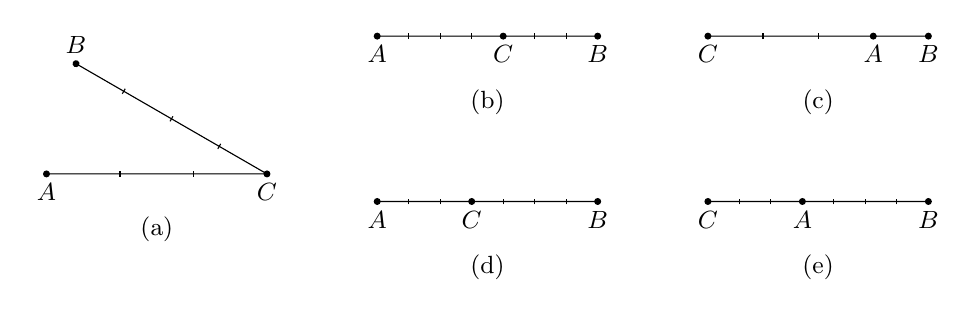
\begin{tikzpicture}[scale=.7,font=\small]
\usetikzlibrary{calc}

\begin{scope}[yshift=-2.5cm,rotate=150]
\coordinate (o) at (0,0);
\draw[fill] (o) -- (4,0) circle (1.5pt) node[above] {$B$};
\foreach \x in {1,2,3}
{
	\draw (\x,-1.5pt) -- (\x,1.5pt);
}
\end{scope}

\begin{scope}[yshift=-2.5cm,xshift=-4cm]
\coordinate (o) at (0,0);
\draw[fill] (o) circle (1.5pt) node[below] {$A$} -- (4,0) circle (1.5pt) node[below] {$C$};
\foreach \x in {1.333,2.666}
{
	\draw (\x,-1.5pt) -- (\x,1.5pt);
}
\node at (2,-1) {(a)};
\end{scope}

\begin{scope}[xshift=2cm]
\coordinate (o) at (0,0);
\draw[fill] (o) circle (1.5pt) node[below] {$A$} -- (4,0) circle (1.5pt) node[below] {$B$};
\foreach \x in {0.57142,1.142857,...,3.428572}
{
	\draw (\x,-1.5pt) -- (\x,1.5pt);
}
\draw[fill] (2.285714,0) circle (1.5pt) node[below] {$C$};
\node at (2,-1.2) {(b)};
\end{scope}

\begin{scope}[xshift=8cm]
\coordinate (o) at (0,0);
\draw[fill] (o) circle (1.5pt) node[below] {$C$} -- (4,0) circle (1.5pt) node[below] {$B$};
\foreach \x in {1,2}
{
	\draw (\x,-1.5pt) -- (\x,1.5pt);
}
\draw[fill] (3,0) circle (1.5pt) node[below] {$A$};
\node at (2,-1.2) {(c)};
\end{scope}

\begin{scope}[xshift=2cm, yshift=-3cm]
\coordinate (o) at (0,0);
\draw[fill] (o) circle (1.5pt) node[below] {$A$} -- (4,0) circle (1.5pt) node[below] {$B$};
\foreach \x in {0.57142,1.142857,...,3.428572}
{
	\draw (\x,-1.5pt) -- (\x,1.5pt);
}
\draw[fill] (1.714285,0) circle (1.5pt) node[below] {$C$};
\node at (2,-1.2) {(d)};
\end{scope}

\begin{scope}[xshift=8cm, yshift=-3cm]
\coordinate (o) at (0,0);
\draw[fill] (o) circle (1.5pt) node[below] {$C$} -- (4,0) circle (1.5pt) node[below] {$B$};
\foreach \x in {0.57142,1.142857,...,3.428572}
{
	\draw (\x,-1.5pt) -- (\x,1.5pt);
}
\draw[fill] (1.714285,0) circle (1.5pt) node[below] {$A$};
\node at (2,-1.2) {(e)};
\end{scope}

\end{tikzpicture}

 \caption{Esercizio~\ref{ese:1.130}}\label{fig:ese1.130}
\end{figure}
\end{inaccessibleblock}

\begin{esercizio}[Prove invalsi 2005]
\label{ese:1.131}
Due segmenti misurano 5~dm e 30~cm rispettivamente. Qual è il 
rapporto fra la lunghezza del secondo segmento e quella del primo?
\begin{multicols}{4}
\begin{enumeratea}
\item 6;
\item $5/3$;
\item $3/5$;
\item $1/6$.
\end{enumeratea}
\end{multicols}
\end{esercizio}

\begin{esercizio}[Prove invalsi 2005]
\label{ese:1.132}
I punti $A$, $B$ e $C$ sono allineati come nella 
figura~\ref{fig:ese1.132}. Se l'angolo $A\widehat{B}E$ misura 
$54\grado$ e $BD$ è la bisettrice dell'angolo $E\widehat{B}C$, quanto 
misura l'angolo $D\widehat{B}C$?
\begin{multicols}{4}
\begin{enumeratea}
\item $26\grado$;
\item $36\grado$;
\item $54\grado$;
\item $63\grado$.
\end{enumeratea}
\end{multicols}
\end{esercizio}


\begin{inaccessibleblock}[Figura: TODO]
 \begin{figure}[htb]
 \centering% Copyright (c) 2015 Daniele Masini - d.masini.it@gmail.com

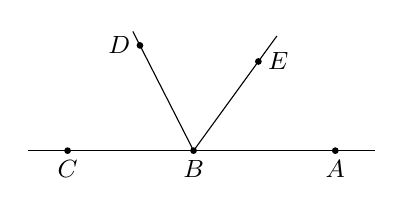
\begin{tikzpicture}[scale=1,font=\small]
\usetikzlibrary{calc}

\begin{scope}
\pgfmathsetmacro{\aalpha}{0};
\pgfmathsetmacro{\abeta}{54};
\pgfmathsetmacro{\agamma}{117};
\pgfmathsetmacro{\adelta}{180};

\draw (0,0) coordinate (b) node[below] {$B$} -- +({\aalpha}:2.3);
\draw[fill] (b) circle (1pt);
\draw[fill] +({\aalpha}:1.8) circle (1pt) node[below] {$A$};
\draw (b) -- +({\abeta}:1.8);
\draw[fill] +({\abeta}:1.4) circle (1pt) node[right] {$E$};
\draw (b) -- +({\agamma}:1.7);
\draw[fill] +({\agamma}:1.5) circle (1pt) node[left] {$D$};
\draw (b) -- +({\adelta}:2.1);
\draw[fill] +({\adelta}:1.6) circle (1pt) node[below] {$C$};
\end{scope}

\end{tikzpicture}

 \caption{Esercizio~\ref{ese:1.132}}\label{fig:ese1.132}
\end{figure}
\end{inaccessibleblock}

%\pagebreak

\begin{esercizio}[Prove invalsi 2005]
\label{ese:1.133}
Un poligono è regolare se tutti i suoi lati sono uguali e tutti i 
suoi angoli sono uguali. Un poligono non è regolare se e solamente se 
\ldots
\begin{enumeratea}
\item tutti i suoi lati e tutti i suoi angoli sono disuguali;
\item tutti i suoi lati o tutti i suoi angoli sono disuguali;
\item almeno due dei suoi lati e almeno due dei suoi angoli sono tra 
loro disuguali;
\item almeno due dei suoi lati o almeno due dei suoi angoli sono tra 
loro disuguali.
\end{enumeratea}
\end{esercizio}


\subsection{Risposte}

\begingroup
\hypersetup{linkcolor=black}

\paragraph{\ref{ese:1.1}.}
a)~F,\quad b)~V,\quad c)~F,\quad d)~V,\quad e)~V,\quad f)~F,\quad 
g)~V,\quad h)~F,\quad i)~F,\quad j)~F,\quad k)~V,\quad l)~V.

\paragraph{\ref{ese:1.3}.}
a)~V,\quad b)~F,\quad c)~F,\quad d)~V,\quad e)~V,\quad f)~F,\quad 
g)~V,\quad h)~V,\quad i)~F,\quad j)~V.

\paragraph{\ref{ese:1.5}.}
a)~$p\wedge q$,\quad b)~$\neg p\wedge q$,\quad c)~$p\wedge \neg 
q$,\quad d)~$\neg p \wedge \neg q$.

\paragraph{\ref{ese:1.6}.}
a)~o escl\@.,\quad b)~o escl\@.,\quad c)~o incl\@.,\quad d)~o 
escl\@.,\quad e)~o escl\@.,\quad f)~o escl.

\paragraph{\ref{ese:1.11}.}
d.

\paragraph{\ref{ese:1.12}.}
a.

\paragraph{\ref{ese:1.13}.}
\begin{enumeratea}
\item <<Al compito di matematica alcuni non erano presenti>>
\item <<Almeno un giorno il professore non ha dato i compiti per 
casa>>
\item <<Almeno un giorno Luca non vede il telegiornale>>
\item <<Almeno uno dei miei familiari non porta gli occhiali>>
\item <<Alcuni non hanno portato i soldi per la gita>>
\end{enumeratea}

\paragraph{\ref{ese:1.14}.}
a)~V,\quad b)~F,\quad c)~F.

\paragraph{\ref{ese:1.18}.}
a)~P,\quad b)~D,\quad c)~D,\quad d)~P,\quad e)~P,\quad f)~D.

\paragraph{\ref{ese:1.19}.}
Un controesempio è 6, che è pari.

\paragraph{\ref{ese:1.20}.}
a.

\paragraph{\ref{ese:1.22}.}
Anna.

\paragraph{\ref{ese:1.23}.}
Bea.

\paragraph{\ref{ese:1.24}.}
e.

\paragraph{\ref{ese:1.25}.}
c.

\paragraph{\ref{ese:1.33}.}
c.

\paragraph{\ref{ese:1.34}.}
c.

\paragraph{\ref{ese:1.35}.}
a)~V,\quad b)~F,\quad c)~V,\quad d)~V,\quad e)~V.

\paragraph{\ref{ese:1.41}.}
a.

\paragraph{\ref{ese:1.49}.}
a)~F,\quad b)~V,\quad c)~F,\quad d)~V,\quad e)~V,\quad f)~F,\quad 
g)~F,\quad h)~F,\quad i)~F,\quad j)~F,\quad k)~F,\quad l)~V.

\paragraph{\ref{ese:1.50}.}
e.

\paragraph{\ref{ese:1.51}.}
e.

\paragraph{\ref{ese:1.52}.}
e.

\paragraph{\ref{ese:1.60}.}
c.

\paragraph{\ref{ese:1.63}.}
Sì.

\paragraph{\ref{ese:1.67}.}
a.

\paragraph{\ref{ese:1.68}.}
b.

\paragraph{\ref{ese:1.69}.}
b.

\paragraph{\ref{ese:1.70}.}
c.

\paragraph{\ref{ese:1.71}.}
e.

\paragraph{\ref{ese:1.72}.}
d.

\paragraph{\ref{ese:1.73}.}
a)~F,\quad b)~F,\quad c)~F,\quad d)~V,\quad e)~F.

\paragraph{\ref{ese:1.74}.}
b.

\paragraph{\ref{ese:1.75}.}
a.

\paragraph{\ref{ese:1.77}.}
a)~F,\quad b)~V,\quad c)~V,\quad d)~V,\quad e)~V,\quad f)~F,\quad 
g)~F.

\paragraph{\ref{ese:1.81}.}
$\frac{4}{3}$.

\paragraph{\ref{ese:1.83}.}
b.

\paragraph{\ref{ese:1.84}.}
$\frac{5}{3}$.

\paragraph{\ref{ese:1.85}.}
a.

\paragraph{\ref{ese:1.86}.}
c.

\paragraph{\ref{ese:1.104}.}
$\np{13,5}$~cm.

\paragraph{\ref{ese:1.106}.}
$\frac{4}{3}$.

\paragraph{\ref{ese:1.107}.}
44~cm.

\paragraph{\ref{ese:1.108}.}
10~m.

\paragraph{\ref{ese:1.109}.}
6~cm.

\paragraph{\ref{ese:1.110}.}
$38\grado 45'$ e $51\grado 15'$.

\paragraph{\ref{ese:1.111}.}
$\frac{3}{7}\pi$ (circa $77\grado 8' 34''$) e $\frac{4}{7}\pi$ (circa 
$102\grado 51' 26''$).
% 77,142857143 e 102,857142857

\paragraph{\ref{ese:1.112}.}
b.

\paragraph{\ref{ese:1.113}.}
a.

\paragraph{\ref{ese:1.114}.}
$90\grado$ e $90\grado$.

\paragraph{\ref{ese:1.115}.}
$\frac{1}{4}$ e $\frac{1}{2}$.

\paragraph{\ref{ese:1.116}.}
$30\grado$.

\paragraph{\ref{ese:1.117}.}
$54\grado$ e $126\grado$.

\paragraph{\ref{ese:1.118}.}
$50\grado$, $66\grado 40'$ e $83\grado 20'$.

\paragraph{\ref{ese:1.119}.}
$80\grado$, $120\grado$ e $160\grado$.

\paragraph{\ref{ese:1.120}.}
$\overline{AB}=10$~cm e $\overline{CD}=14$~cm.

\paragraph{\ref{ese:1.121}.}
$30$~cm e $42$~cm.

\paragraph{\ref{ese:1.122}.}
$\frac{64}{7}$~cm e $\frac{83}{7}$~cm.

\paragraph{\ref{ese:1.123}.}
45~cm e 57~cm.

\paragraph{\ref{ese:1.124}.}
24~cm e 35~cm.

\paragraph{\ref{ese:1.125}.}
a.

\paragraph{\ref{ese:1.126}.}
d.

\paragraph{\ref{ese:1.128}.}
a)~V,\quad b)~V,\quad c)~V,\quad d)~V,\quad e)~F,\quad f)~F,\quad 
g)~F,\quad h)~F,\quad i)~F.

\paragraph{\ref{ese:1.129}.}
a.

\paragraph{\ref{ese:1.130}.}
d.

\paragraph{\ref{ese:1.131}.}
c.

\paragraph{\ref{ese:1.132}.}
d.

\paragraph{\ref{ese:1.133}.}
d.

\endgroup
